\section{Модальный регулятор}
Рассмотрим систему: 
\begin{equation}
    \dot{x} = Ax + Bu
\end{equation}
где 
\begin{equation}
    \begin{array}{cc}
        A = \begin{bmatrix}
            8 & 1 & 11 \\ 
            4 & 0 & 4 \\
            -4 & -3 & -7
        \end{bmatrix}, &
        B = \begin{bmatrix}
            -1 \\ -3 \\ 3
        \end{bmatrix}
    \end{array}
\end{equation}

\subsection{Управляемость собственных чисел}

Для определения управляемости собственных чисел рассмотрим вещественную Жорданову форму системы: 
\begin{equation}
    \dot{\hat{x}} = P^{-1}AP\hat{x} + P^{-1}Bu
\end{equation}
Где $P$ -- матрица собственных векторов матрицы $A$, а $\hat{x} = P^{-1}x$.
\begin{equation}
    A_j = \begin{bmatrix}
        -3  & 0  & 0 \\ 
        0  & 2  & -2 \\ 
        0  & 2  & 2 \\ 
    \end{bmatrix}\quad
    P = \begin{bmatrix}
        -1  & -2.12  & 0.71 \\ 
        0  & -1.41  & 0 \\ 
        1  & 1.41  & 0 \\ 
    \end{bmatrix}\quad 
    B_j = \begin{bmatrix}
        0 \\ 
        2.12 \\ 
        4.95 \\ 
    \end{bmatrix}
\end{equation}

Таким образом, последнее собственное число $\lambda_3 = -3$ не является управляемым. Соответственно, система не является полностью управляемой. 
Но, так как данное собственное число располагается в левой полуплоскости, то есть является устойчивым, то система является стабилизируемой. 

\subsection{Степень устойчивости}
Так как собственное число $\lambda_3 = -3$ не является управляемым, то добиться степени устойчивости $\alpha > 3$ не удастся, 
так как регулятор не сможем его вывести в устойчивую область. При этом любое значение устойчивости $\alpha \le 3$ является достижимым.

\subsection{Синтез регулятора}
Будем рассматривать два значения степени устойчивости: $\alpha_1 = 3$ и $\alpha_2 = 1$, 
первое из которых является предельным значением, а второе -- достижимым. 
Синтезируем регулятор вида $u = Kx$, который обеспечивает устойчивость системы с заданной степенью устойчивости $\alpha$.

Схема моделирования системы, замкнутой регулятором, представлена на рисунке \ref{fig:scheme1}.
\begin{figure}[ht!]
    \centering
    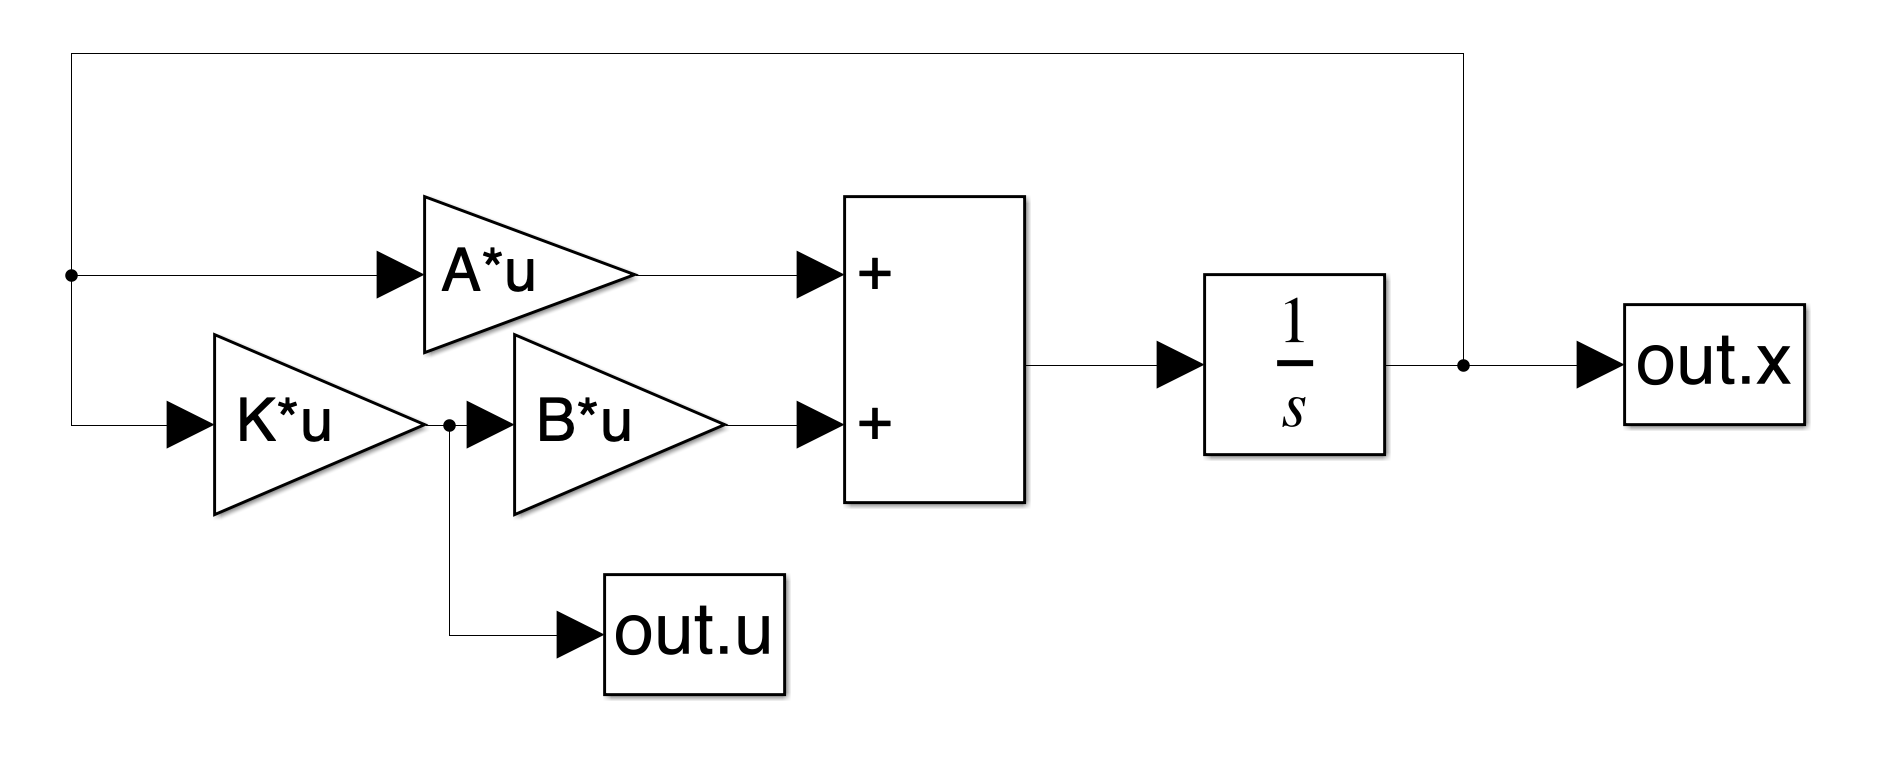
\includegraphics[width=\textwidth]{media/scheme1.png}
    \caption{Схема моделирования системы с регулятором}
    \label{fig:scheme1}
\end{figure}

\subsubsection{Матричноное неравенство Ляпунова}
Рассмотрим матричное неравенство Ляпунова для регулятора:
\begin{equation}
    PA^T + AP + 2\alpha P + Y^T B^T + BY \preceq 0, ~~~ K = Y P^{-1}, ~~~ P \succ 0
\end{equation}
Для решения данного неравенства воспользуемся пакетом \texttt{cvx} в MATLAB. 

Получаем матрицы регулятора для $\alpha_1 = 3$ и $\alpha_2 = 1$:
\begin{equation}
    K_{\alpha_1} = 
    \begin{bmatrix}
        -17.49  & -1.51  & -14.88 \\ 
    \end{bmatrix}
\end{equation}
\begin{equation}
    K_{\alpha_2} = 
    \begin{bmatrix}
        -10.83  & -1.32  & -10.95 \\ 
    \end{bmatrix}
\end{equation}

Проверим спектры систем, замкнутых данными регуляторами. Для этого найдем собственные 
числа матрицы $\sigma_i = A + BK_{\alpha_i}$ для каждого из регуляторов.
\begin{equation}
    \sigma_1 = \begin{bmatrix}
        -9.30 + 10.44j \\ 
        -9.30 - 10.44j \\ 
        -3.00 \\ 
    \end{bmatrix}
\end{equation}
\begin{equation}
    \sigma_2 = \begin{bmatrix}
        -7.02 + 6.91j \\ 
        -7.02 - 6.91j \\ 
        -3.00 \\ 
    \end{bmatrix}
\end{equation}
Видим, что степень устойчивости обоих систем получилось равной 3, 
что удовлетворяет заданным степеням устойчивости. При этом, остальные, более удаленные 
от мнимой оси собственные числа меньше при большей заданной степени устойчивости, 
но в обоих случаях не являются максимально возможными с сохранением поставленных условий.

Проведем моделирование систем, замкнутых регуляторами $K_{\alpha_1}$ и $K_{\alpha_2}$,
при начальном состоянии $x(0) = \begin{bmatrix}1 & 1 & 1\end{bmatrix}^T$. 
Результаты моделирования представлены на рисунках \ref{fig:task1_1_x} и \ref{fig:task1_1_u} 
(графики состояния и управления соответственно) для первого регулятора и на рисунках \ref{fig:task1_2_x} и \ref{fig:task1_2_u} 
(графики состояния и управления соответственно) для второго регулятора.
\begin{figure}[ht!]
    \centering
    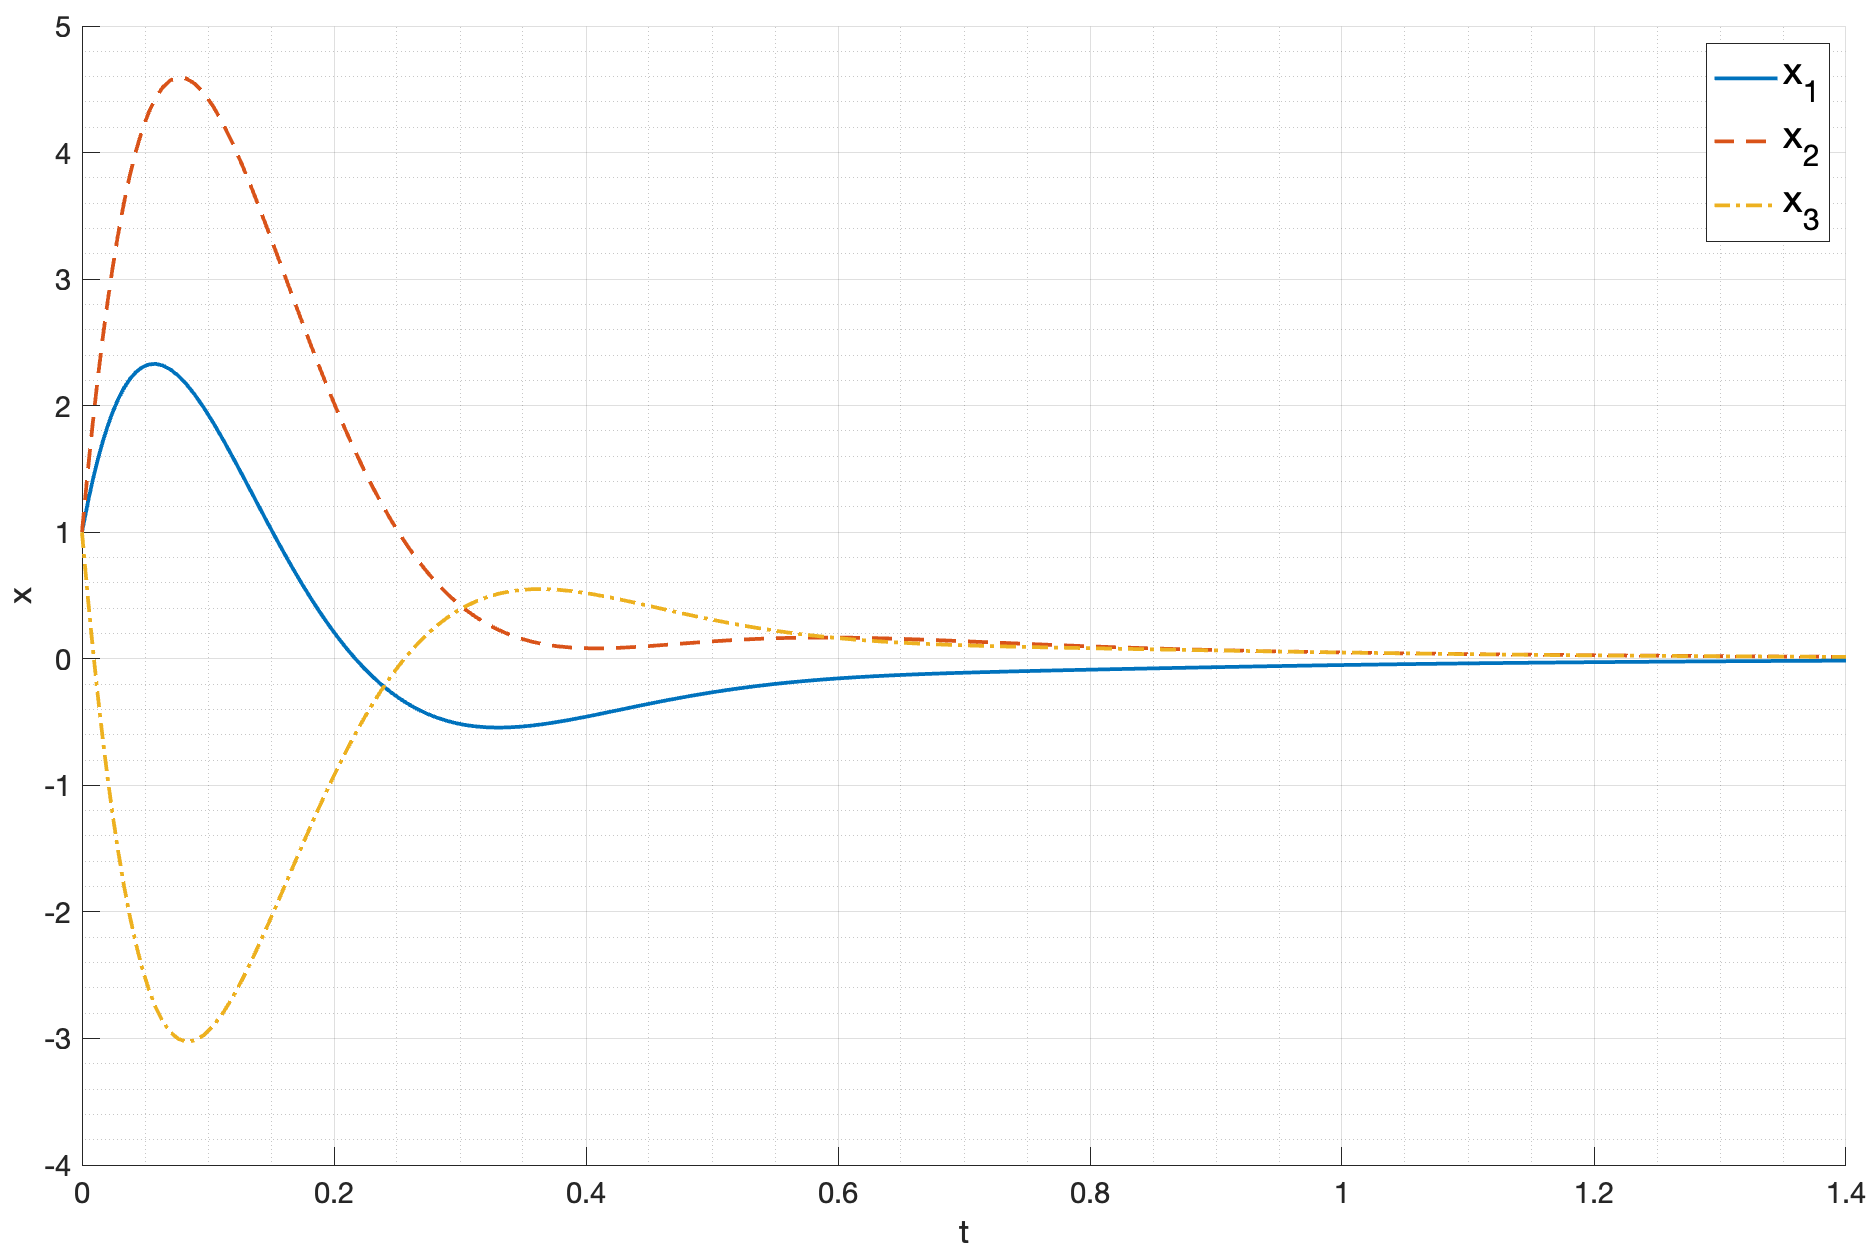
\includegraphics[width=\textwidth]{media/plots/task1_1_x.png}
    \caption{График состояния системы с регулятором $K_{\alpha_1}$}
    \label{fig:task1_1_x}
\end{figure}
\begin{figure}[ht!]
    \centering
    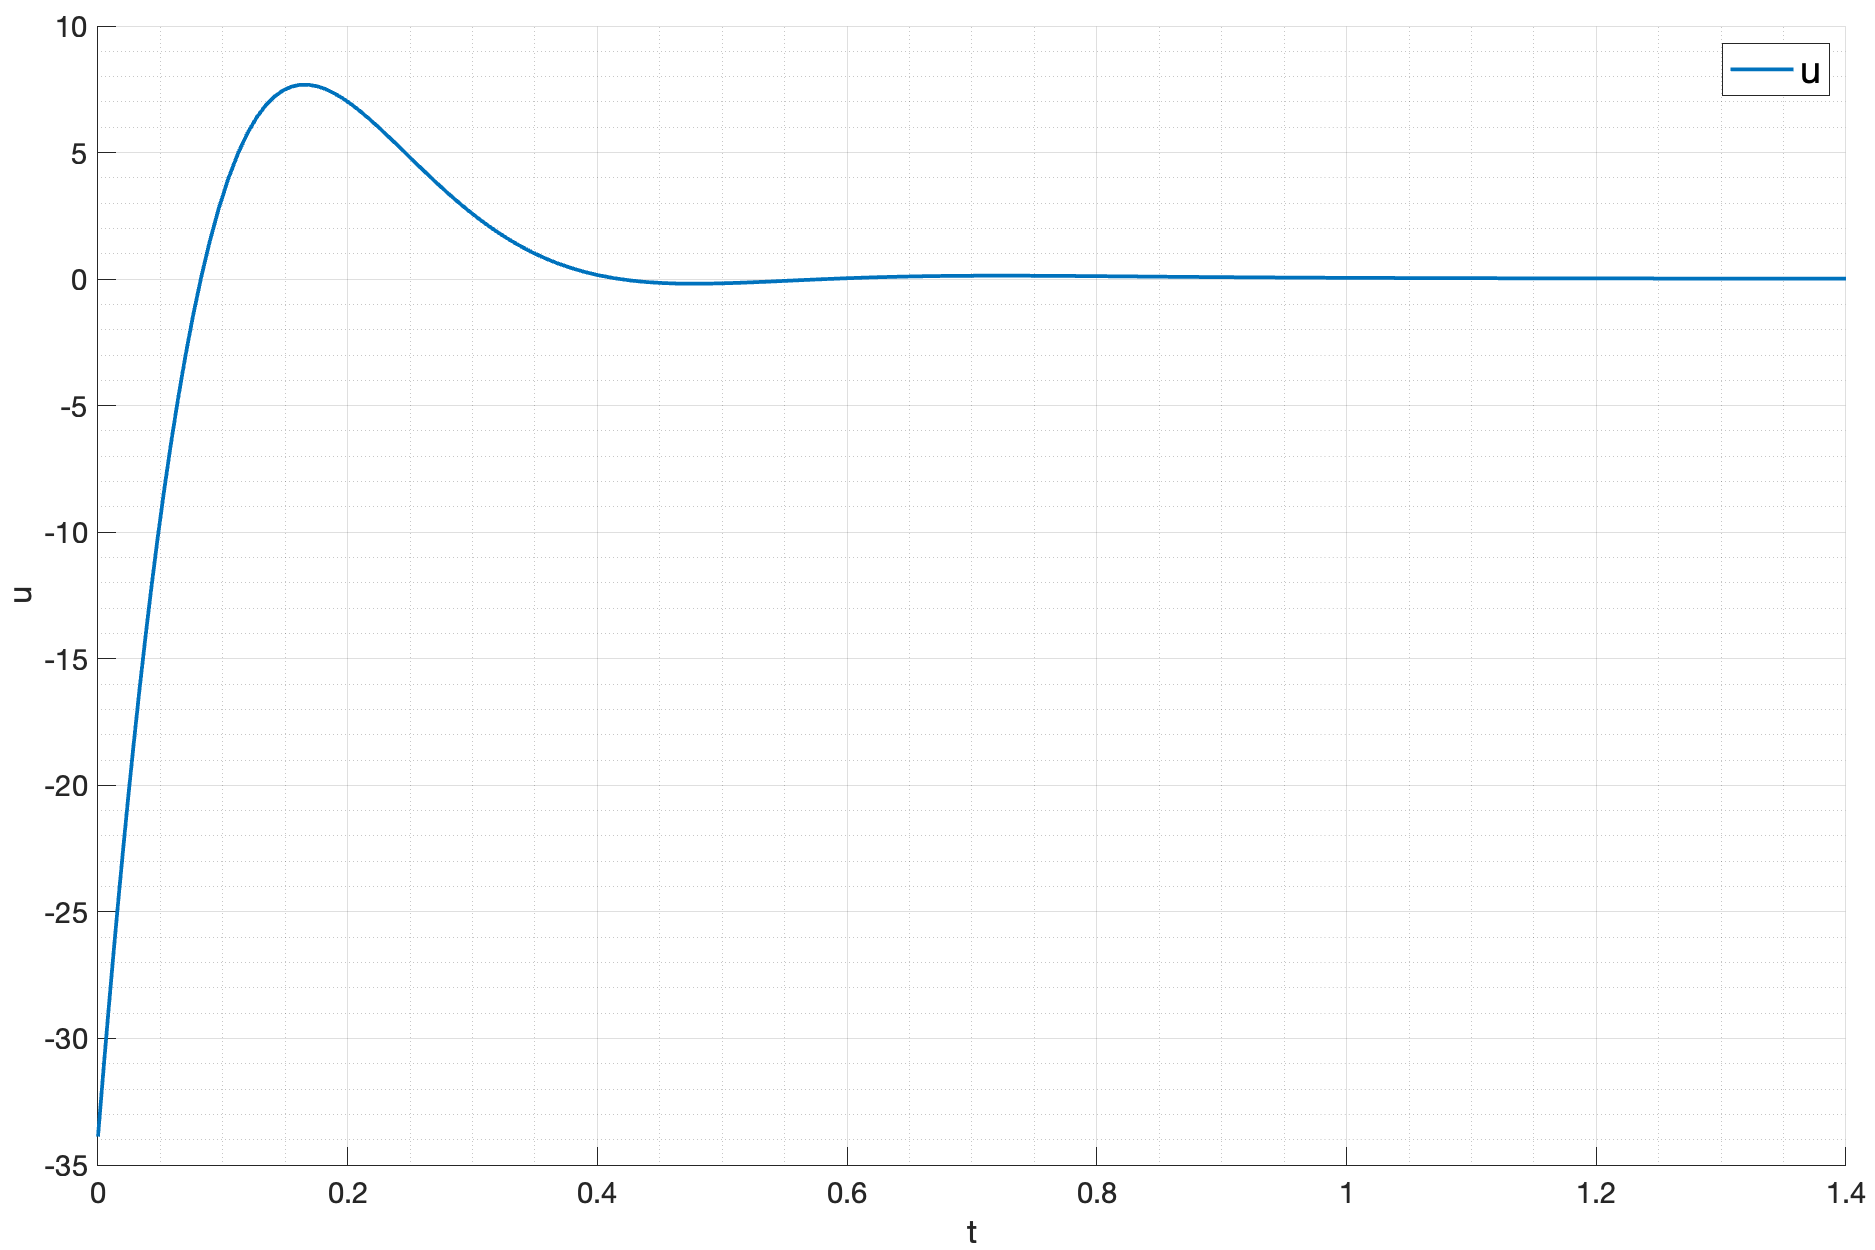
\includegraphics[width=\textwidth]{media/plots/task1_1_u.png}
    \caption{График управления системой с регулятором $K_{\alpha_1}$}
    \label{fig:task1_1_u}
\end{figure}
\begin{figure}[ht!]
    \centering
    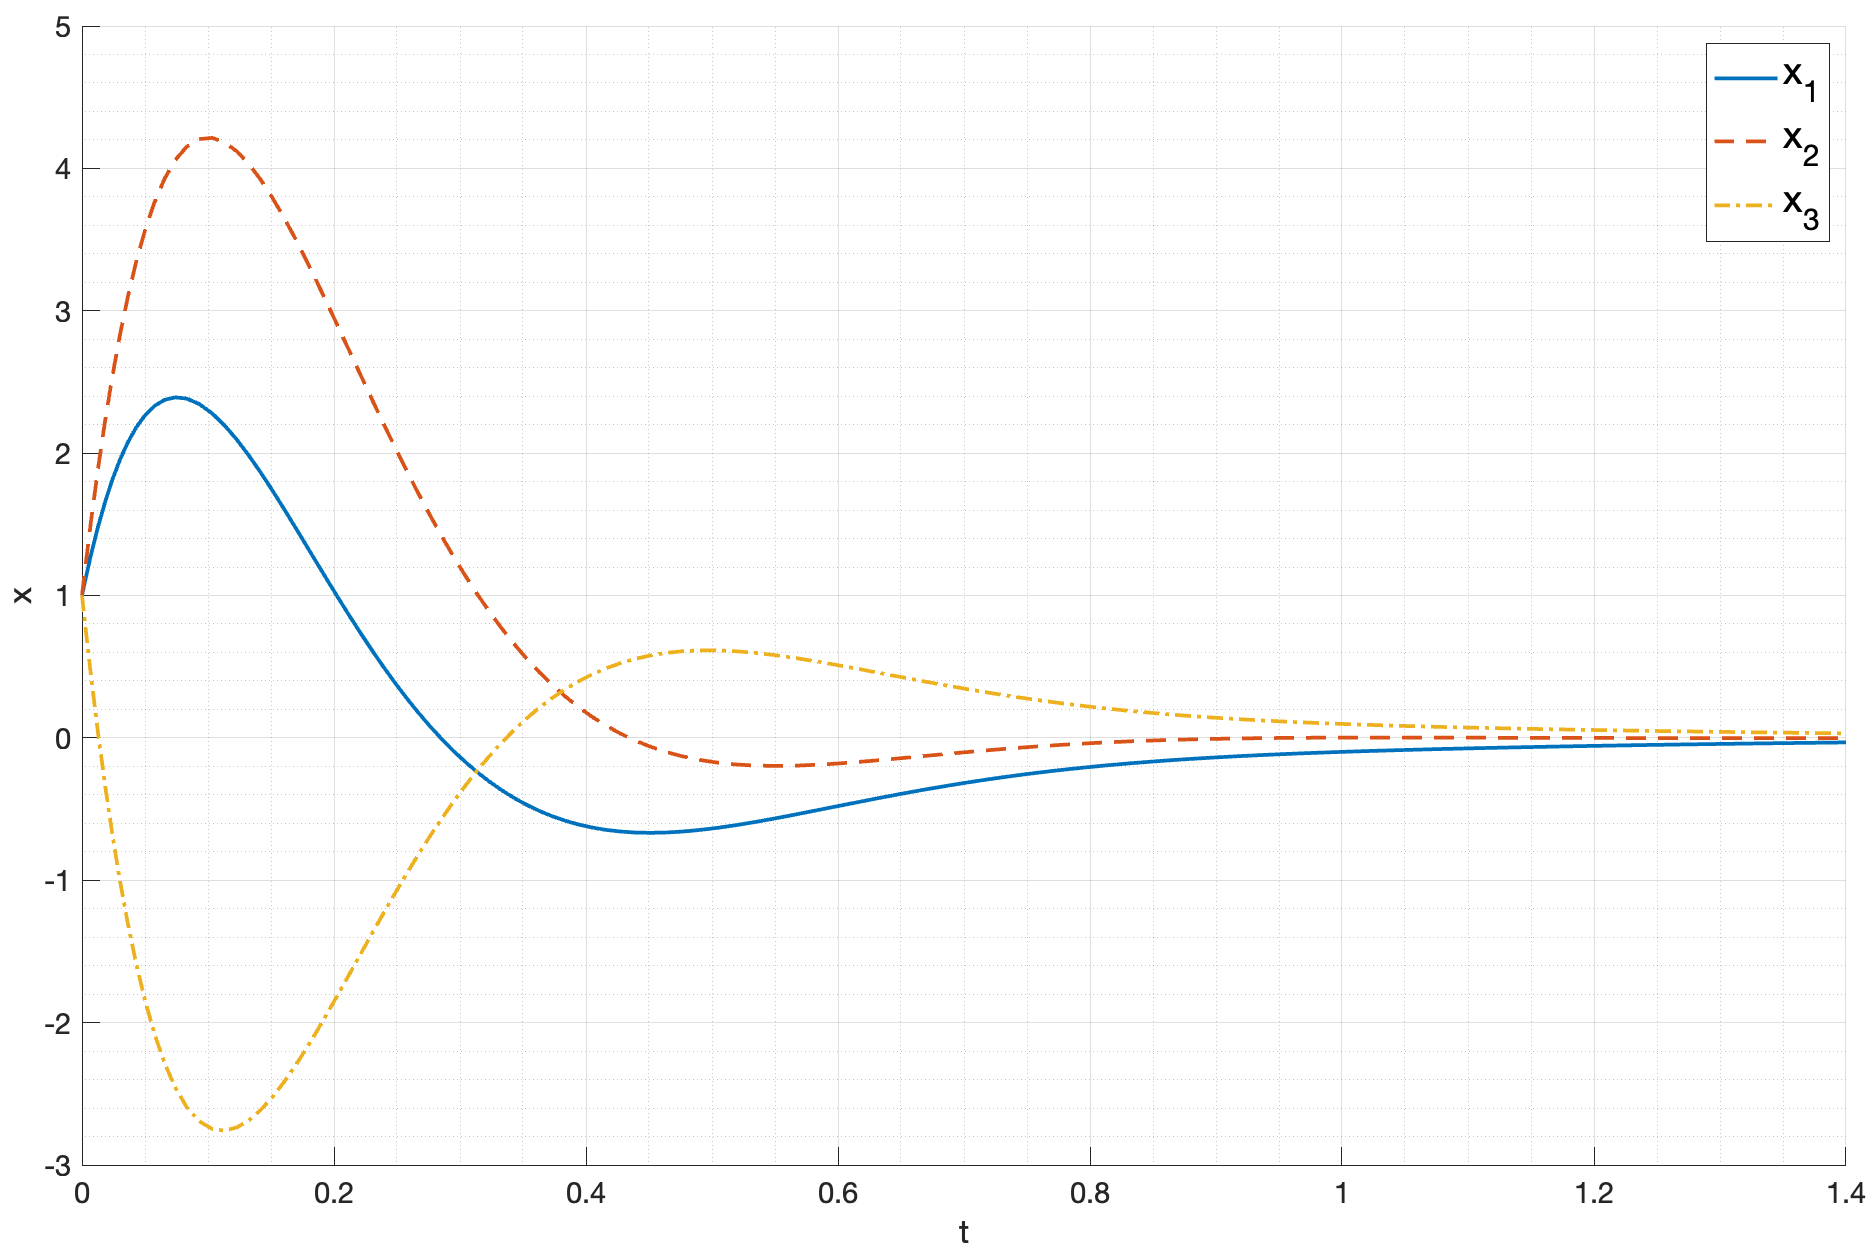
\includegraphics[width=\textwidth]{media/plots/task1_2_x.png}
    \caption{График состояния системы с регулятором $K_{\alpha_2}$}
    \label{fig:task1_2_x}
\end{figure}
\begin{figure}[ht!]
    \centering
    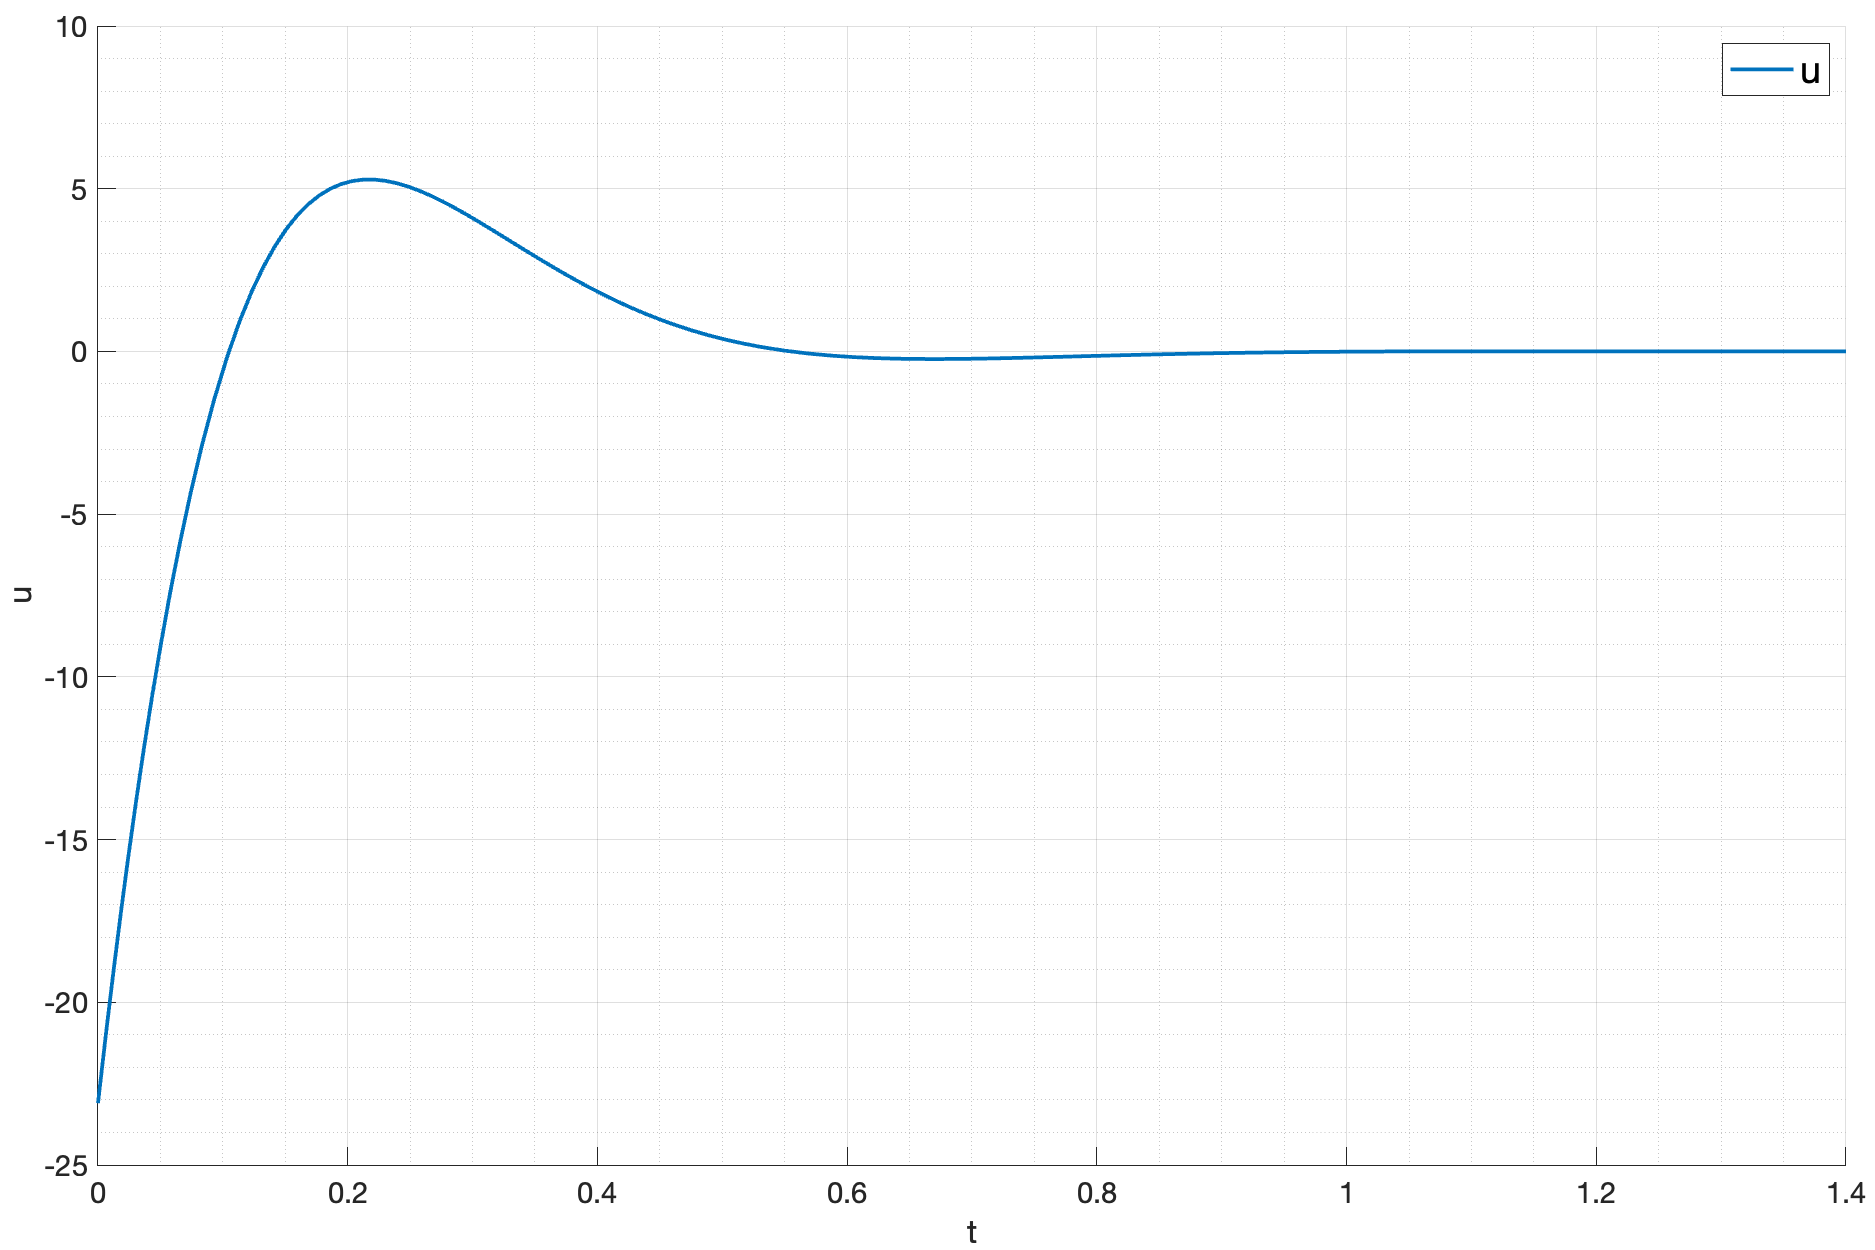
\includegraphics[width=\textwidth]{media/plots/task1_2_u.png}
    \caption{График управления системой с регулятором $K_{\alpha_2}$}
    \label{fig:task1_2_u}
\end{figure}
\FloatBarrier

\subsubsection{Матричное неравенство Ляпунова с минимизацией управления}
Рассмотрим такую же задачу нахождения регулятора $H$, обеспечивающего заданную степень устойчивости 
системы, но теперь добавим условие минимальности управления. Неравенства в данном случае 
будут следующими:
\begin{equation}
    \begin{array}{cc}
        PA^T + AP + 2\alpha P + Y^T B^T + BY \preceq 0, ~~~ H = Y P^{-1}, ~~~ P \succ 0 \\ 
        \begin{bmatrix}
            P & x(0) \\
            x(0)^T & 1
        \end{bmatrix} \succ 0, ~~~ \begin{bmatrix}
            P & Y^T \\
            Y & \mu^2I
        \end{bmatrix} \succ 0
    \end{array}
\end{equation} 
где $\mu$ -- ограничение на управление $\mu \ge \|u(t)\|_2$.

Минимизируя $\mu$ при заданной степени устойчивости $\alpha$ и начальном 
состоянии $x(0) = \begin{bmatrix}1 & 1 & 1\end{bmatrix}^T$, получаем следующие 
матрицы регуляторов:
\begin{equation}
    H_{\alpha_1} = \begin{bmatrix}
        -4.45  & 0.37  & -4.44 \\ 
    \end{bmatrix}
\end{equation}
\begin{equation}
    H_{\alpha_2} = \begin{bmatrix}
        -2.18  & 0.55  & -2.18 \\ 
    \end{bmatrix}
\end{equation}
И спектры систем, замкнутых данными регуляторами:
\begin{equation}
    \sigma_1 = \begin{bmatrix}
        -3.00 + 4.29j \\ 
        -3.00 - 4.29j \\ 
        -3.00 \\ 
    \end{bmatrix}
\end{equation}
\begin{equation}
    \sigma_2 = \begin{bmatrix}
        -1.00 + 3.02j \\ 
        -1.00 - 3.02j \\ 
        -3.00 \\ 
    \end{bmatrix}
\end{equation}

В данном случае, в отличие от прошлого, степень устойчивости систем, замкнутых 
регулятором с оптимизацией управления, в точности равна заданной степени устойчивости. 

При этом, в ходе расчетов, были получены значения ограничения на управление $\mu_1$ и $\mu_2$ 
соответственно: 
\begin{equation}
    \begin{array}{cc}
        \mu_1 = 11.974878 & \mu_2 = 5.126559 \\  
    \end{array}
\end{equation}
Ожидаемо, с более строгими ограничениями на степень сходимости, ограничение на 
управление системы становится слабее. 

Проведем моделирование систем, замкнутых регуляторами $H_{\alpha_1}$ и $H_{\alpha_2}$,
при начальном состоянии $x(0) = \begin{bmatrix}1 & 1 & 1\end{bmatrix}^T$.
Результаты моделирования представлены на рисунках \ref{fig:task1_3_x} и \ref{fig:task1_3_u} 
(графики состояния и управления соответственно) для первого регулятора и на рисунках \ref{fig:task1_4_x} и \ref{fig:task1_4_u} 
(графики состояния и управления соответственно) для второго регулятора.

\begin{figure}[ht!]
    \centering
    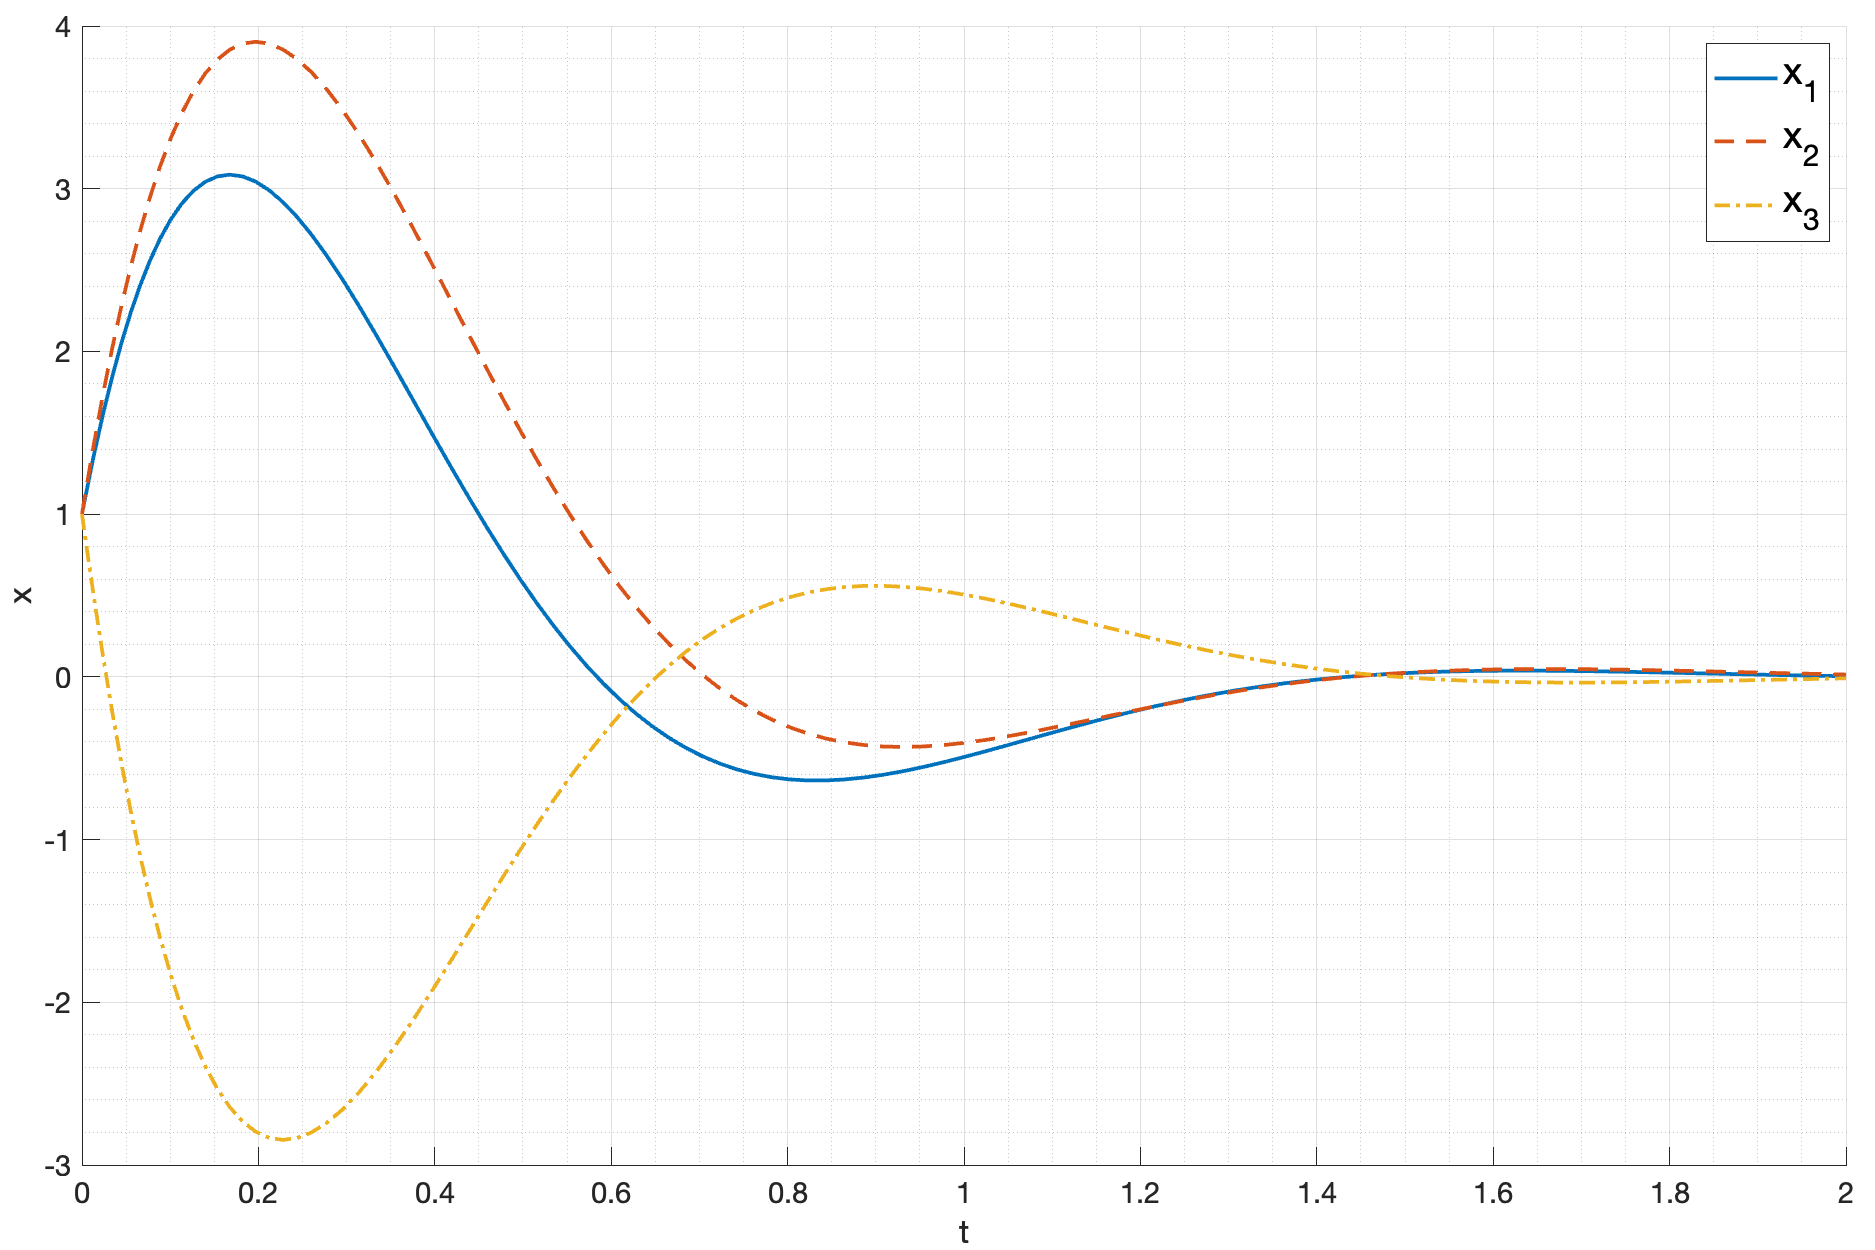
\includegraphics[width=\textwidth]{media/plots/task1_3_x.png}
    \caption{График состояния системы с регулятором $H_{\alpha_1}$}
    \label{fig:task1_3_x}
\end{figure}
\begin{figure}[ht!]
    \centering
    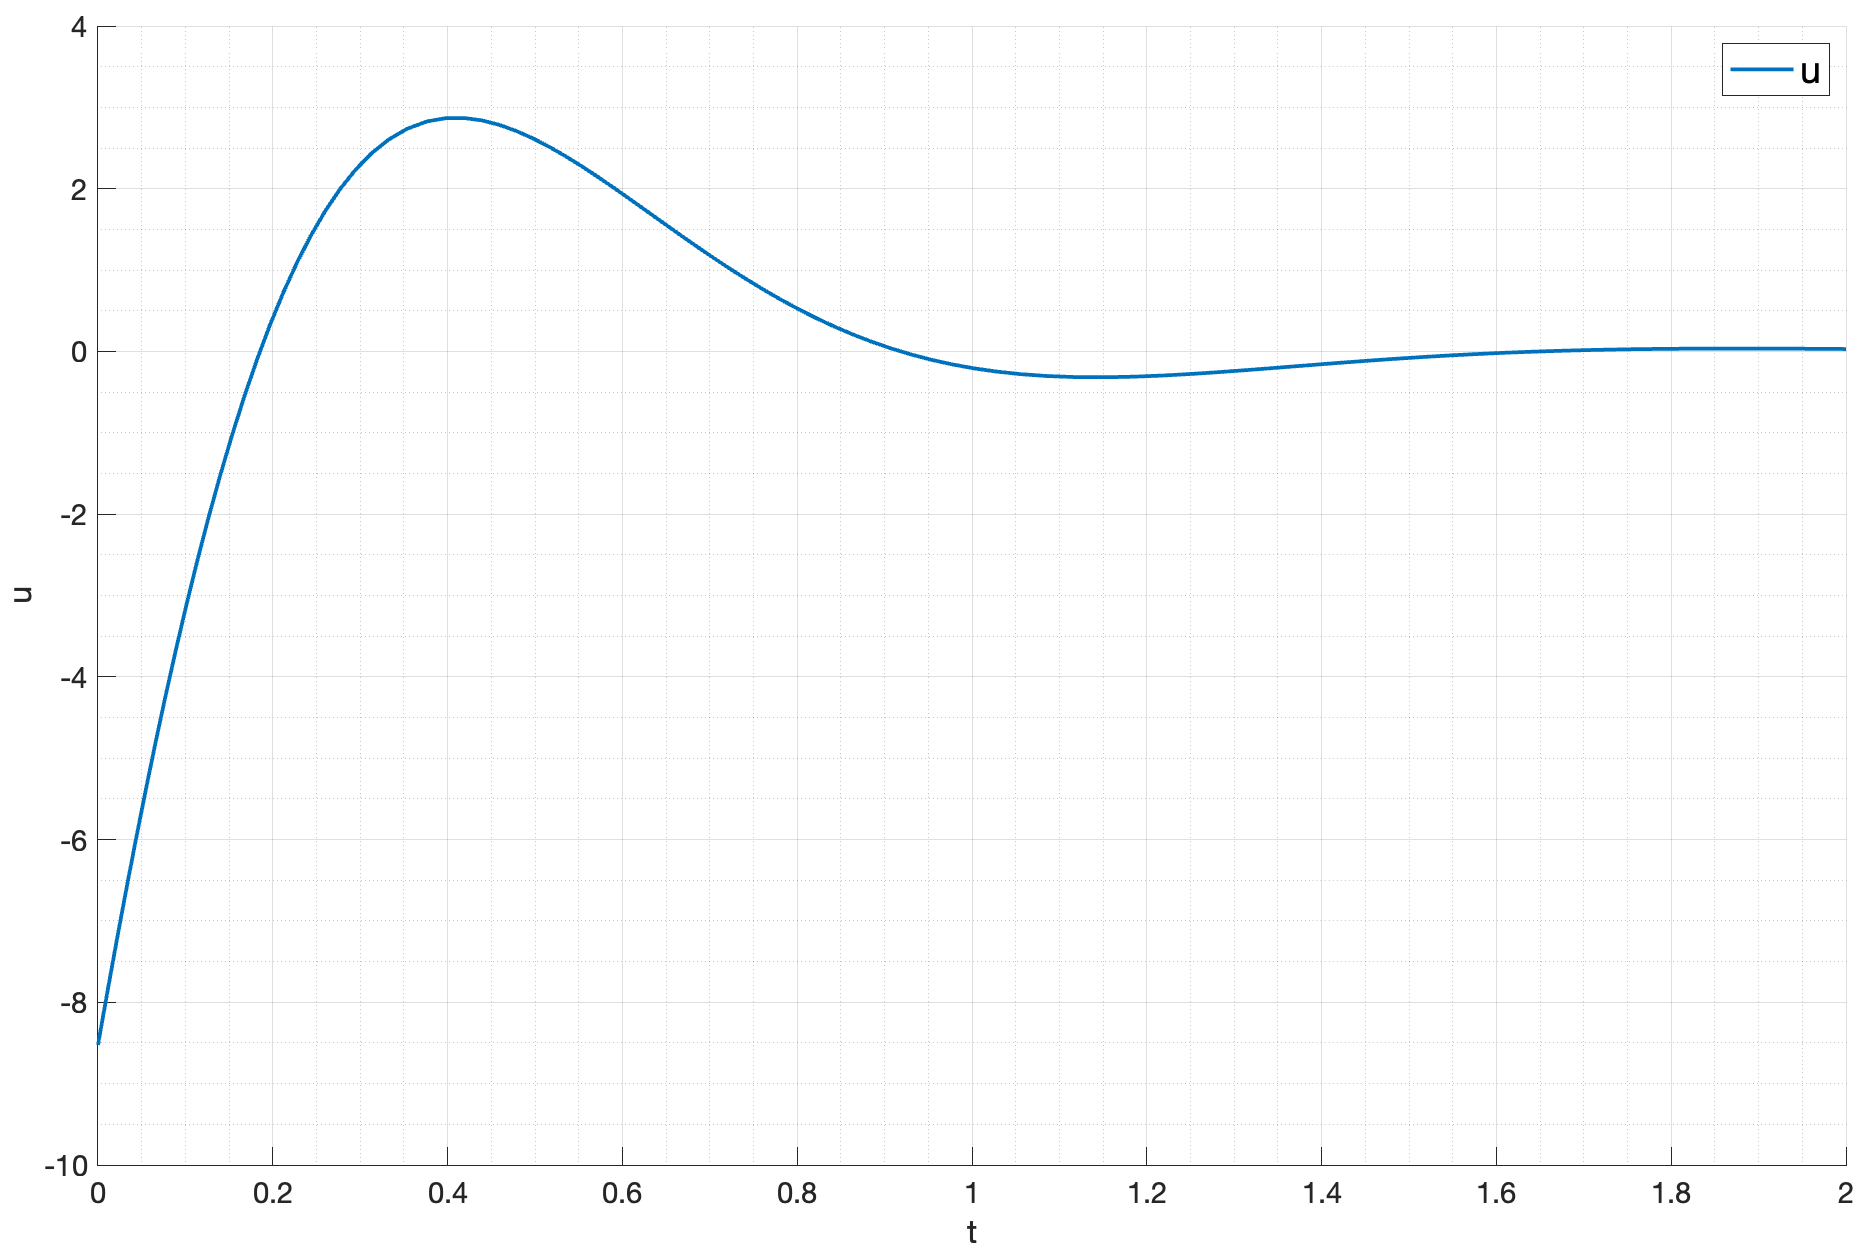
\includegraphics[width=\textwidth]{media/plots/task1_3_u.png}
    \caption{График управления системой с регулятором $H_{\alpha_1}$}
    \label{fig:task1_3_u}
\end{figure}
\begin{figure}[ht!]
    \centering
    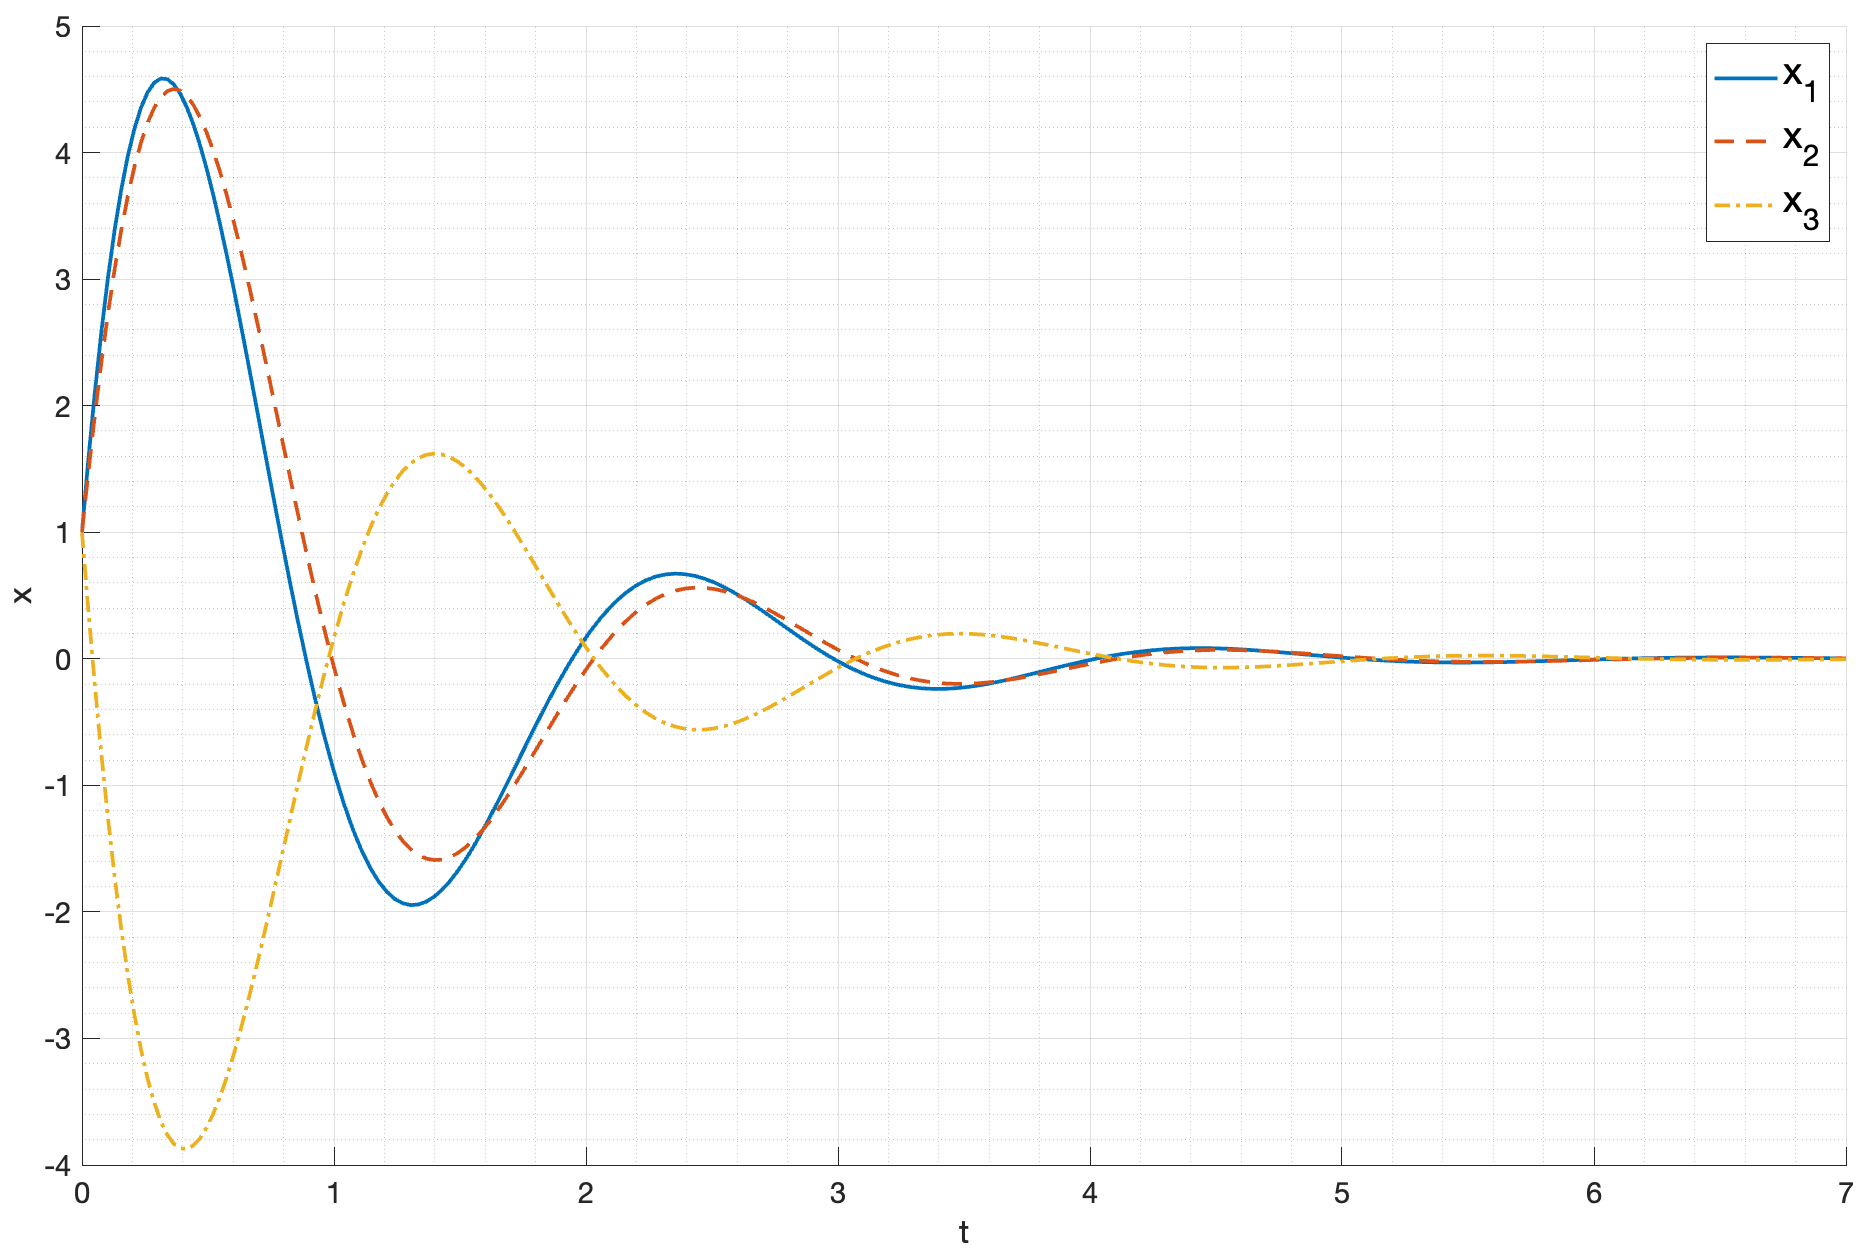
\includegraphics[width=\textwidth]{media/plots/task1_4_x.png}
    \caption{График состояния системы с регулятором $H_{\alpha_2}$}
    \label{fig:task1_4_x}
\end{figure}
\begin{figure}[ht!]
    \centering
    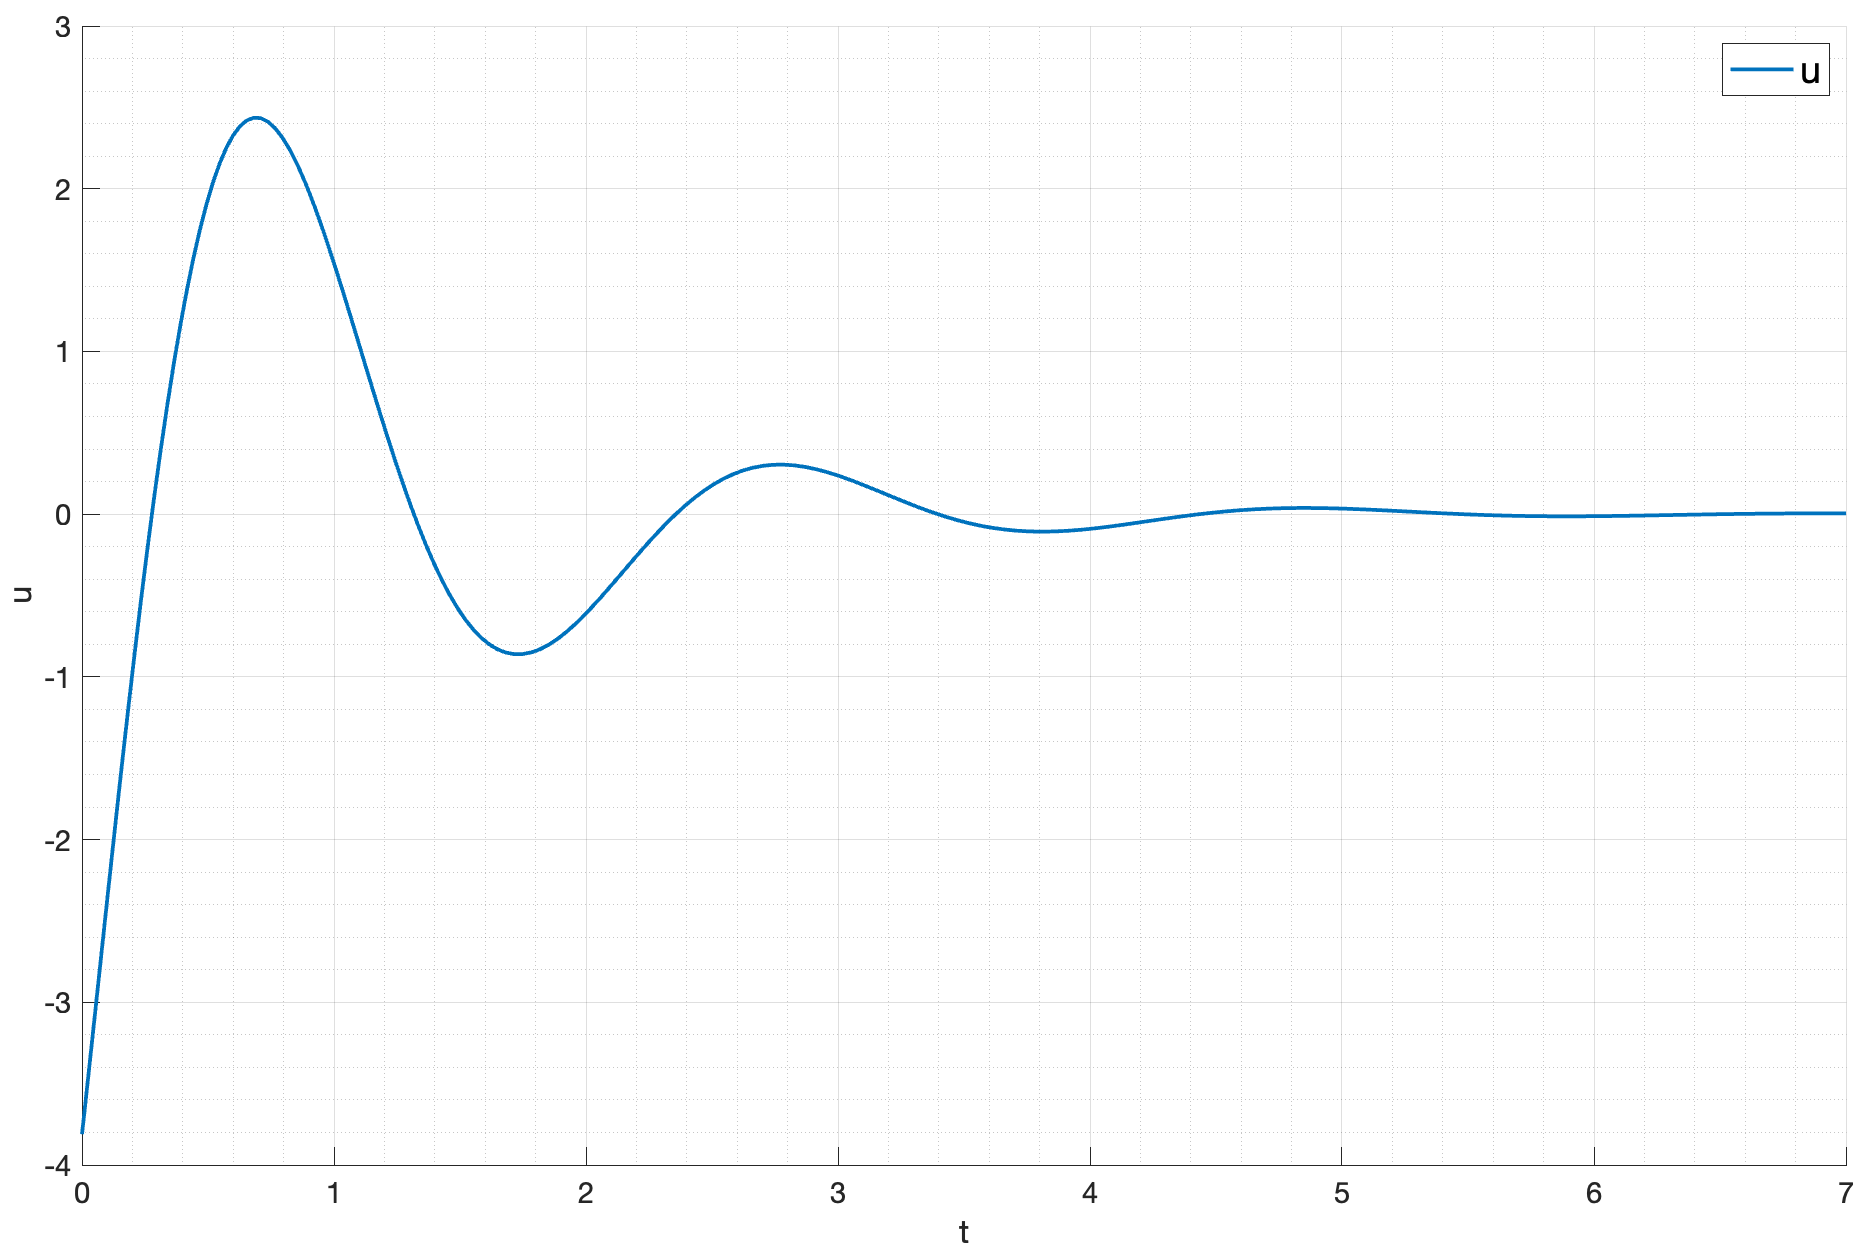
\includegraphics[width=\textwidth]{media/plots/task1_4_u.png}
    \caption{График управления системой с регулятором $H_{\alpha_2}$}
    \label{fig:task1_4_u}
\end{figure}

\FloatBarrier   

Вследствие того, что степень устойчивости системы, замкнутой регулятором $H_{\alpha_1}$, 
больше, чем у системы, замкнутой регулятором $K_{\alpha_1}$, состояния системы с регулятором $H_{\alpha_1}$
сходятся быстрее, чем с регулятором $K_{\alpha_1}$.
При этом, управление системой с регулятором $H_{\alpha_1}$ также меньше, чем с регулятором $K_{\alpha_1}$. 
Можно заметить, что в обоих случаях управление по модулю не превосходит $\mu_1$ и $\mu_2$ соответственно, 
что говорит о том, что полученные теоретически ограничения на управление выполняются.

\FloatBarrier
\subsubsection{Матричное уравнение Риккати}
Теперь рассмотрим синтез регулятора с помощью матричного уравнения Риккати при 
$v = 2$ и $R = 1$.
\begin{equation}
    A^TP + PA + Q - vPBR^{-1}B^TP + 2\alpha P \preceq 0, ~~~ P \succ 0, ~~~ K = -R^{-1}B^TP 
\end{equation}
Решение данного уравнения также будет получено с помощью функции \texttt{icare} в MATLAB.

Найдем матрицы регуляторов $K_3$, $K_4$ для $\alpha_1 = 3$ для $Q = I$ и $Q = 0$ соответственно.
\begin{equation}
    K_3 = \begin{bmatrix}
        -7.54  & -0.06  & -6.79 \\ 
    \end{bmatrix}
\end{equation}
\begin{equation}
    K_4 = \begin{bmatrix}
        -3.77  & -0.09  & -3.39 \\ 
    \end{bmatrix}
\end{equation}
Спектры систем, замкнутых данными регуляторами:
\begin{equation}
    \sigma_3 = \begin{bmatrix}
        -4.31 + 7.14j \\ 
        -4.31 - 7.14j \\ 
        -3.00 \\ 
    \end{bmatrix}
\end{equation}
\begin{equation}
    \sigma_4 = \begin{bmatrix}
        -2.99 + 5.38j \\ 
        -2.99 - 5.38j \\ 
        -3.00 \\ 
    \end{bmatrix}
\end{equation}

В первом случае, при $Q = I$, степень устойчивости двух управляемых собственных чисел системы 
оказывается больше заданной степени устойчивости $\alpha_1 = 3$. Во втором случае, при $Q = 0$,
степень устойчивости двух управляемых собственных чисел системы оказывается равной заданной степени устойчивости $\alpha_1 = 3$.

Проведем моделирование систем, замкнутых регуляторами $K_3$ и $K_4$,
при начальном состоянии $x(0) = \begin{bmatrix}1 & 1 & 1\end{bmatrix}^T$.
Результаты моделирования представлены на рисунках \ref{fig:task1_5_x} и \ref{fig:task1_5_u} 
(графики состояния и управления соответственно) для первого регулятора и на рисунках \ref{fig:task1_6_x} и \ref{fig:task1_6_u} 
(графики состояния и управления соответственно) для второго регулятора.
\begin{figure}[ht!]
    \centering
    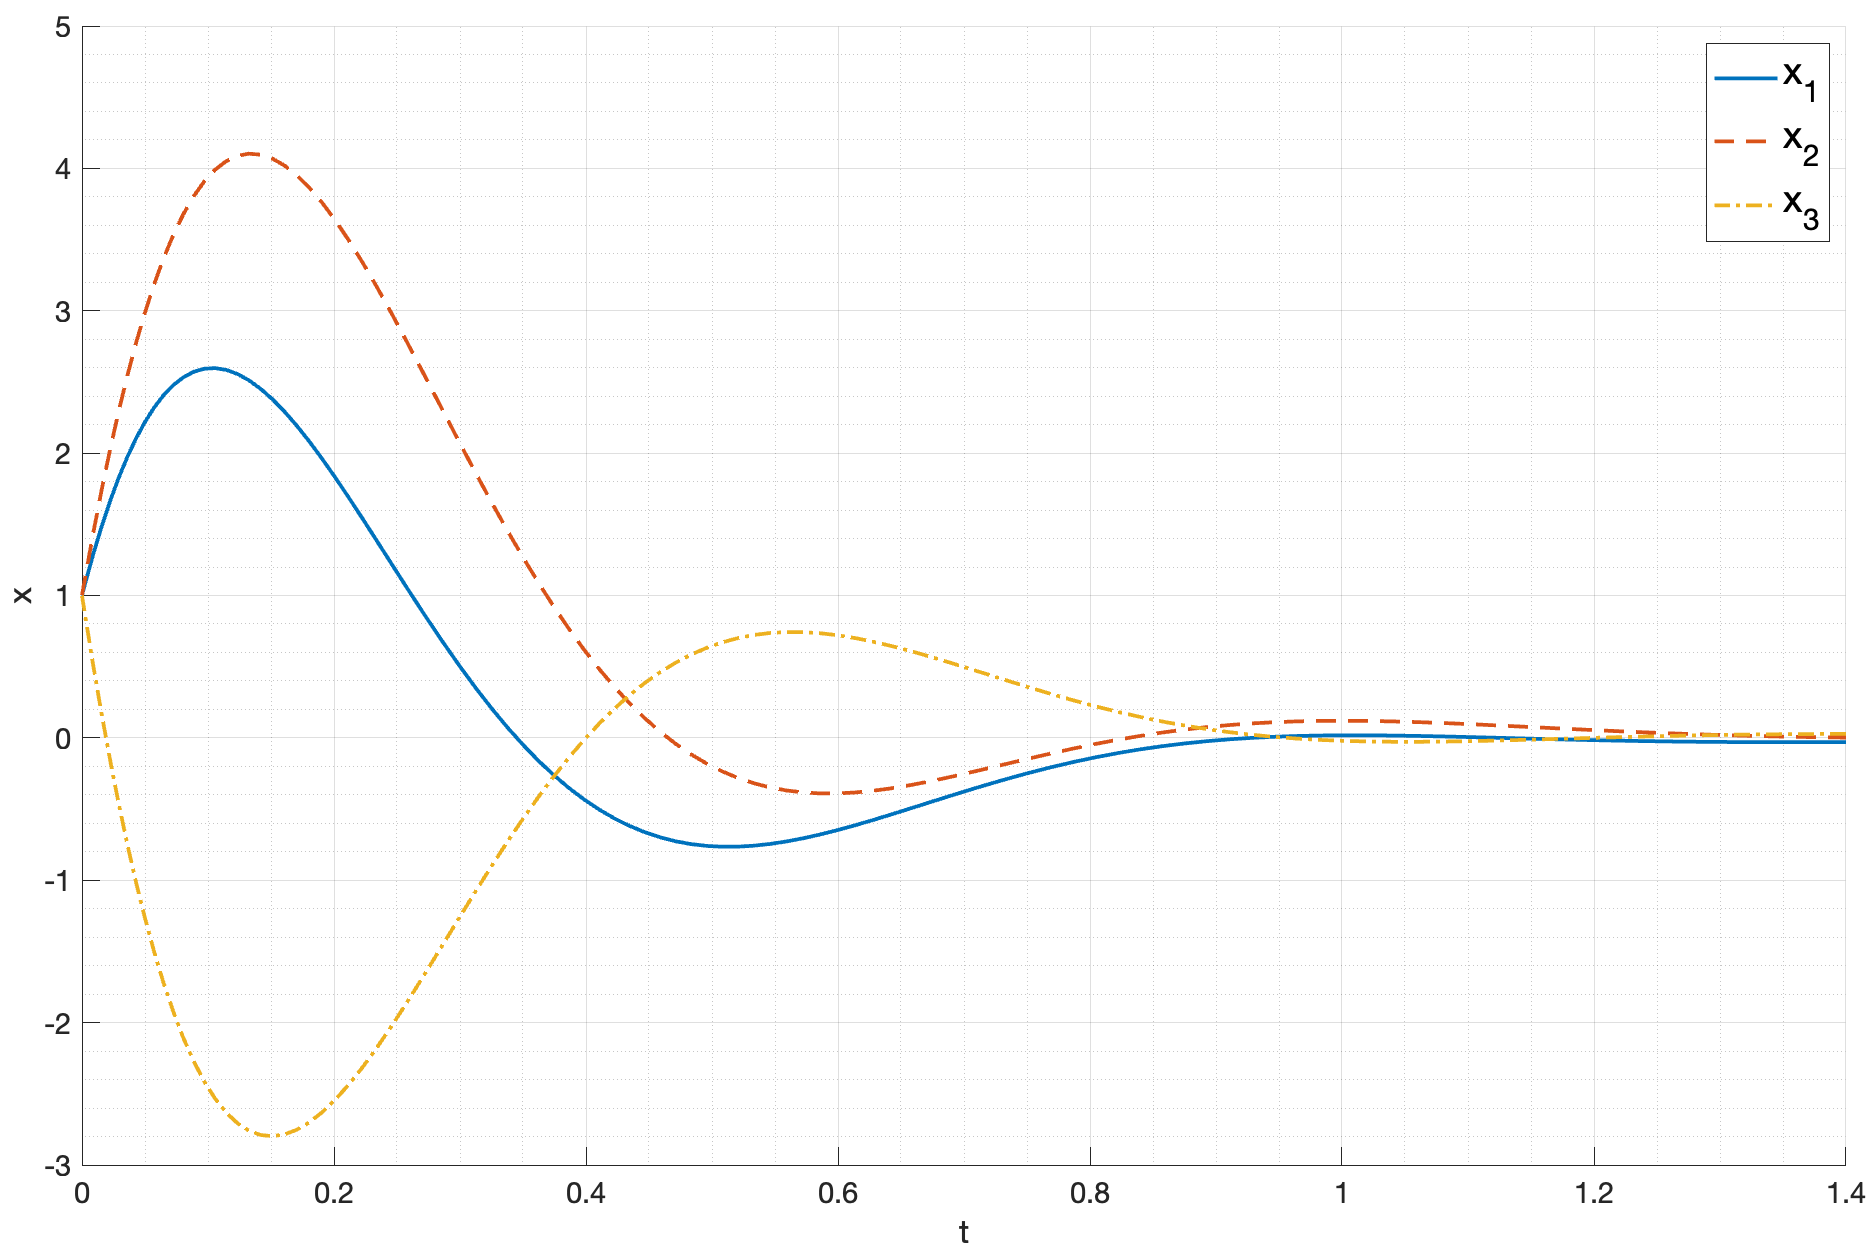
\includegraphics[width=\textwidth]{media/plots/task1_5_x.png}
    \caption{График состояния системы с регулятором $K_3$}
    \label{fig:task1_5_x}
\end{figure}
\begin{figure}[ht!]
    \centering
    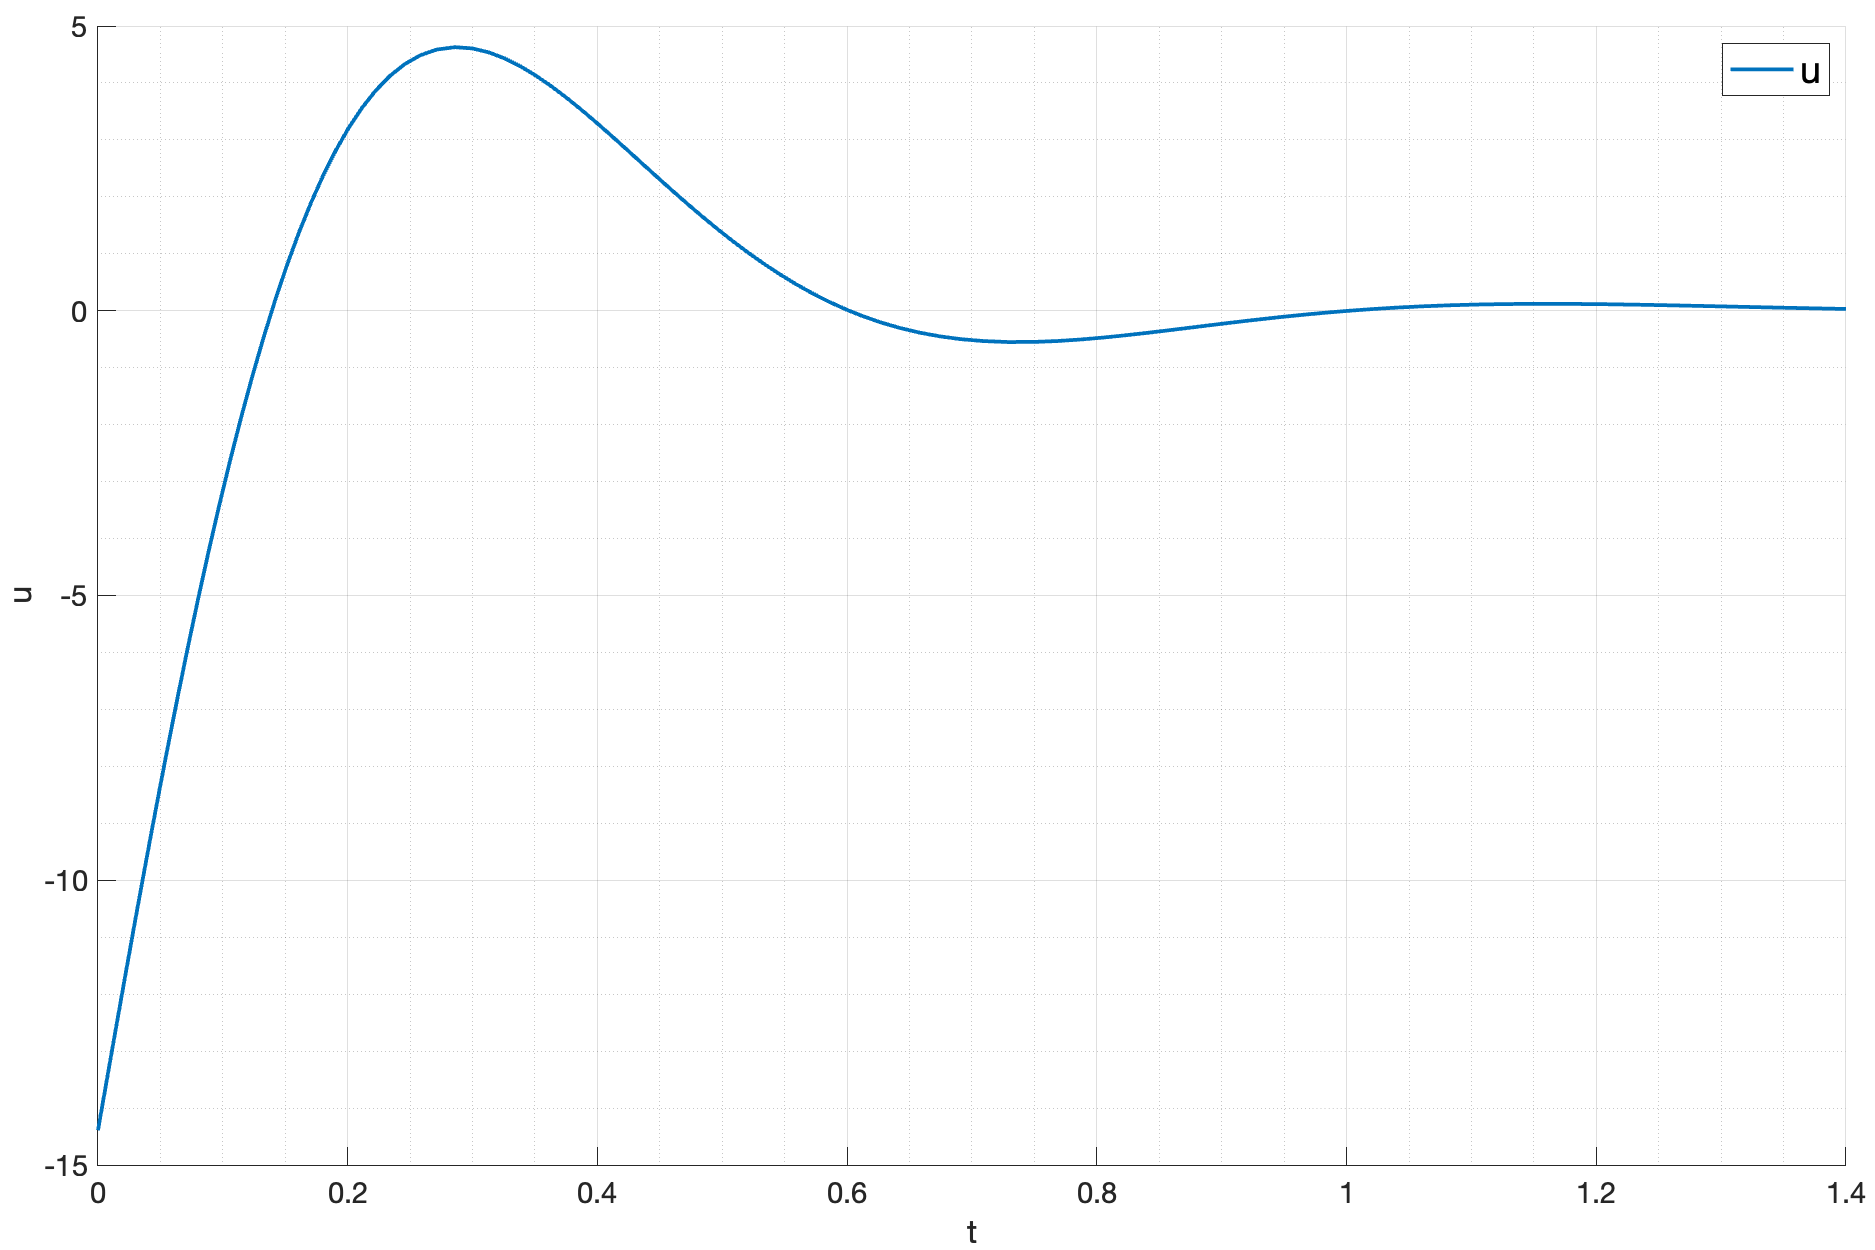
\includegraphics[width=\textwidth]{media/plots/task1_5_u.png}
    \caption{График управления системой с регулятором $K_3$}
    \label{fig:task1_5_u}
\end{figure}
\begin{figure}[ht!]
    \centering
    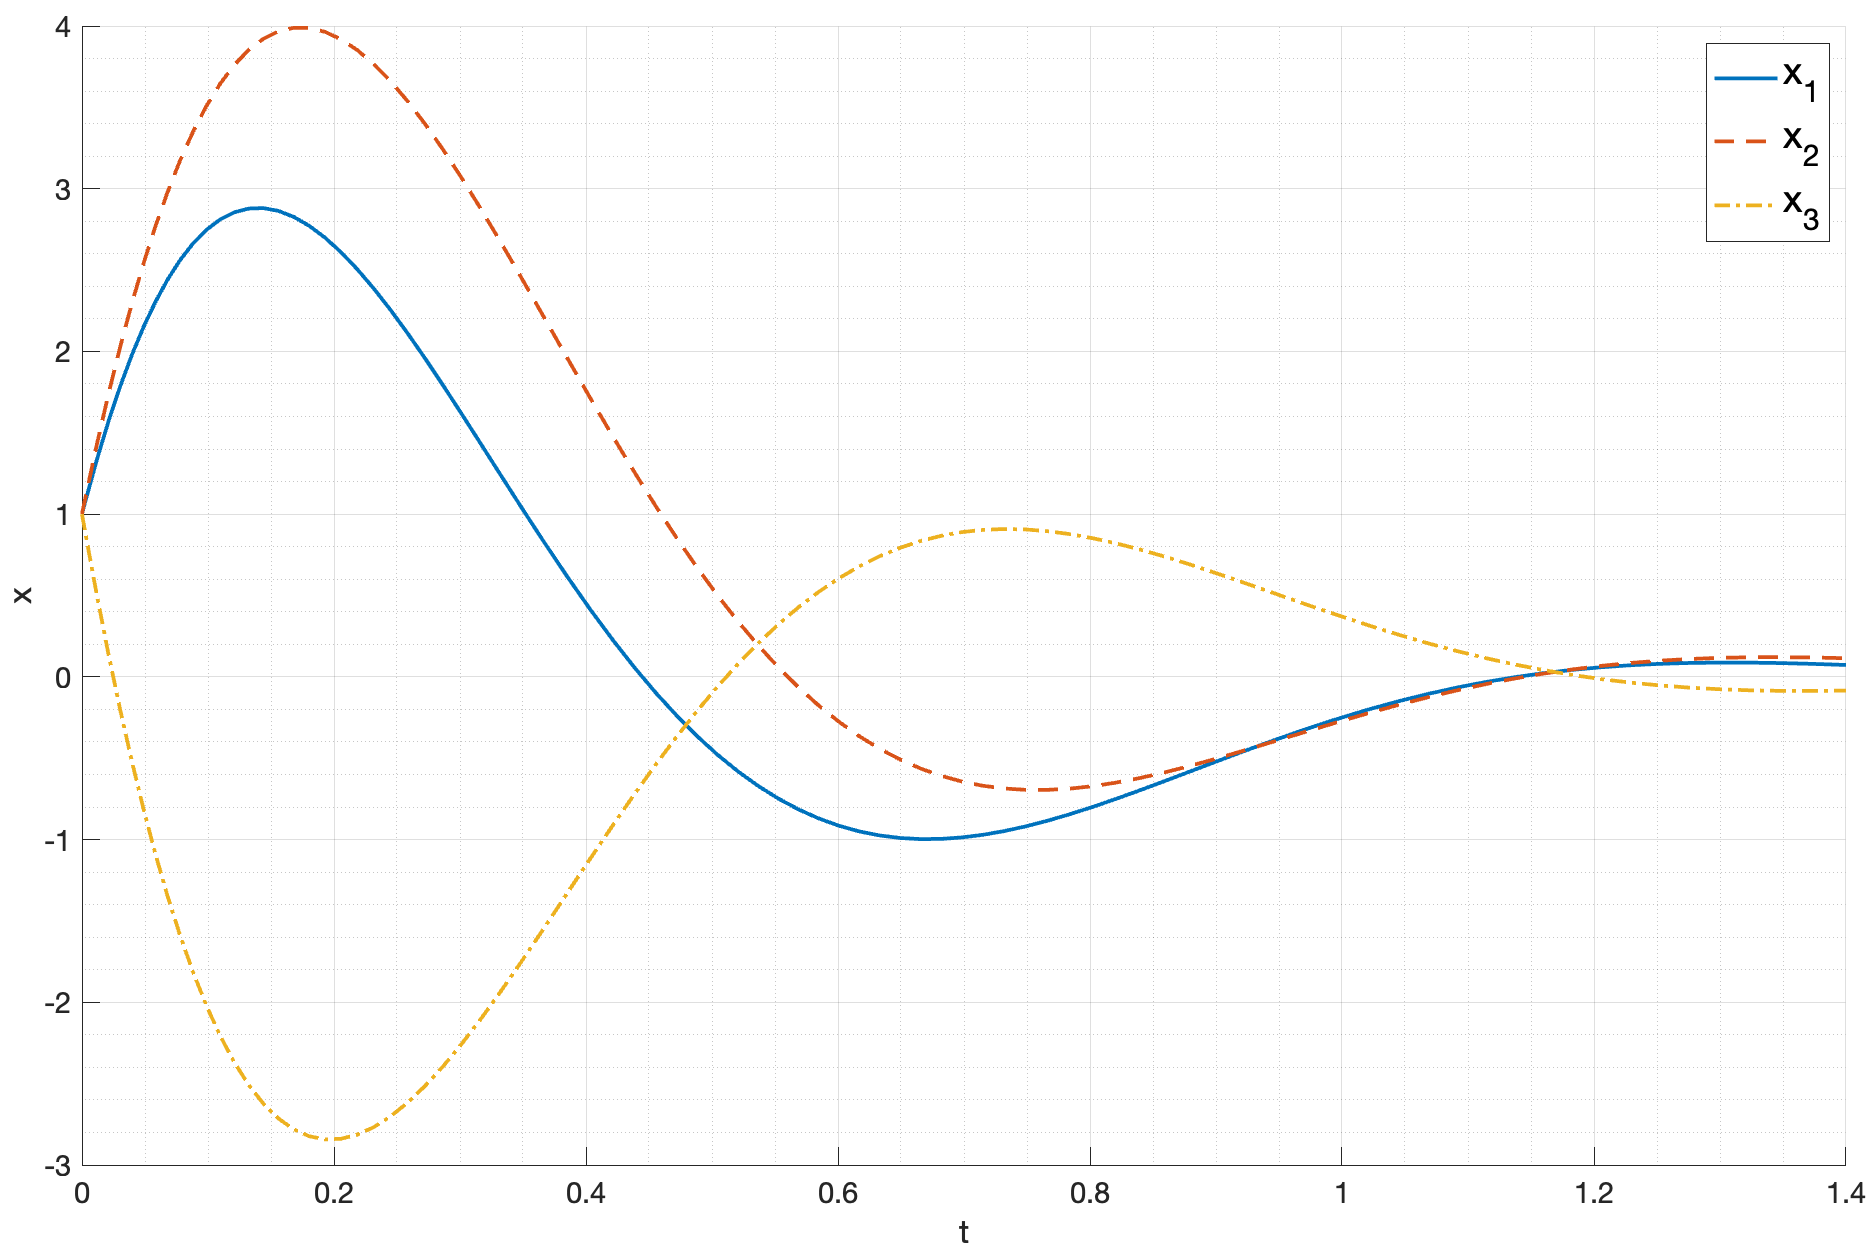
\includegraphics[width=\textwidth]{media/plots/task1_6_x.png}
    \caption{График состояния системы с регулятором $K_4$}
    \label{fig:task1_6_x}
\end{figure}
\begin{figure}[ht!]
    \centering
    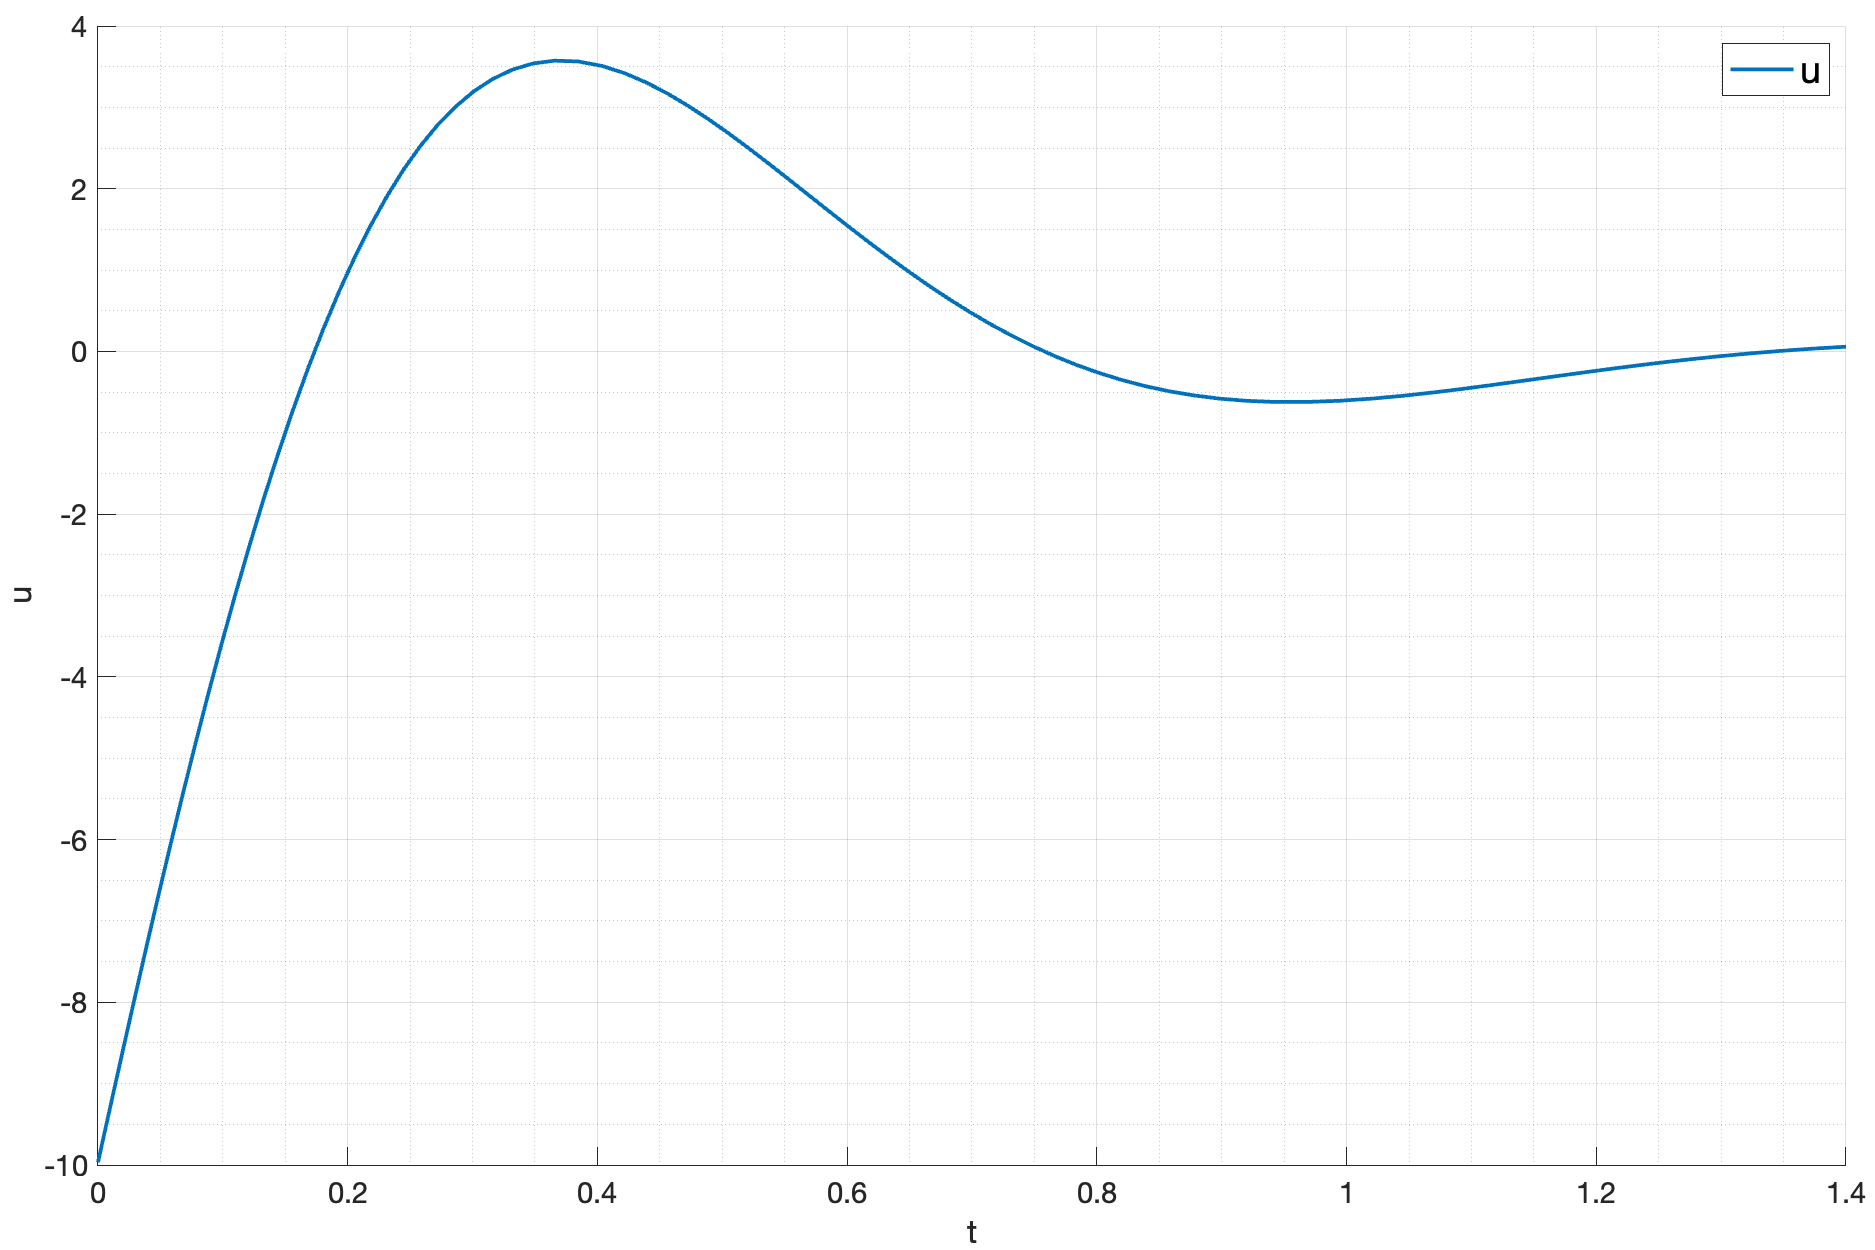
\includegraphics[width=\textwidth]{media/plots/task1_6_u.png}
    \caption{График управления системой с регулятором $K_4$}
    \label{fig:task1_6_u}
\end{figure}

\FloatBarrier

Те же действия повторим для второго спектра и регуляторов $K_5$, $K_6$ для $\alpha_2 = 1$ для $Q = I$ и $Q = 0$ соответственно.
\begin{equation}
    K_5 = \begin{bmatrix}
        -5.01  & 0.29  & -4.55 \\ 
        \end{bmatrix}
\end{equation}
\begin{equation}
    K_6 = \begin{bmatrix}
        -2.37  & 0.41  & -2.37 \\ 
    \end{bmatrix}
\end{equation}

Спектры систем, замкнутых данными регуляторами:
\begin{equation}
    \sigma_5 = \begin{bmatrix}
        -2.76 + 5.82j \\ 
        -2.76 - 5.82j \\ 
        -3.00 \\ 
    \end{bmatrix}
\end{equation}
\begin{equation}
    \sigma_6 = \begin{bmatrix}
        -0.99 + 3.60j \\ 
        -0.99 - 3.60j \\ 
        -3.00 \\ 
    \end{bmatrix}
\end{equation}

Как и в случае с регуляторами $K_3$ и $K_4$, в первом случае, при $Q = I$, степень устойчивости двух управляемых собственных чисел системы
оказывается больше заданной степени устойчивости $\alpha_2 = 1$. Во втором случае, при $Q = 0$,
степень устойчивости двух управляемых собственных чисел системы оказывается равной заданной степени устойчивости $\alpha_2 = 1$.

Проведем моделирование систем, замкнутых регуляторами $K_5$ и $K_6$,
при начальном состоянии $x(0) = \begin{bmatrix}1 & 1 & 1\end{bmatrix}^T$.
Результаты моделирования представлены на рисунках \ref{fig:task1_7_x} и \ref{fig:task1_7_u} 
(графики состояния и управления соответственно) для первого регулятора и на рисунках \ref{fig:task1_8_x} и \ref{fig:task1_8_u} 
(графики состояния и управления соответственно) для второго регулятора.

\begin{figure}[ht!]
    \centering
    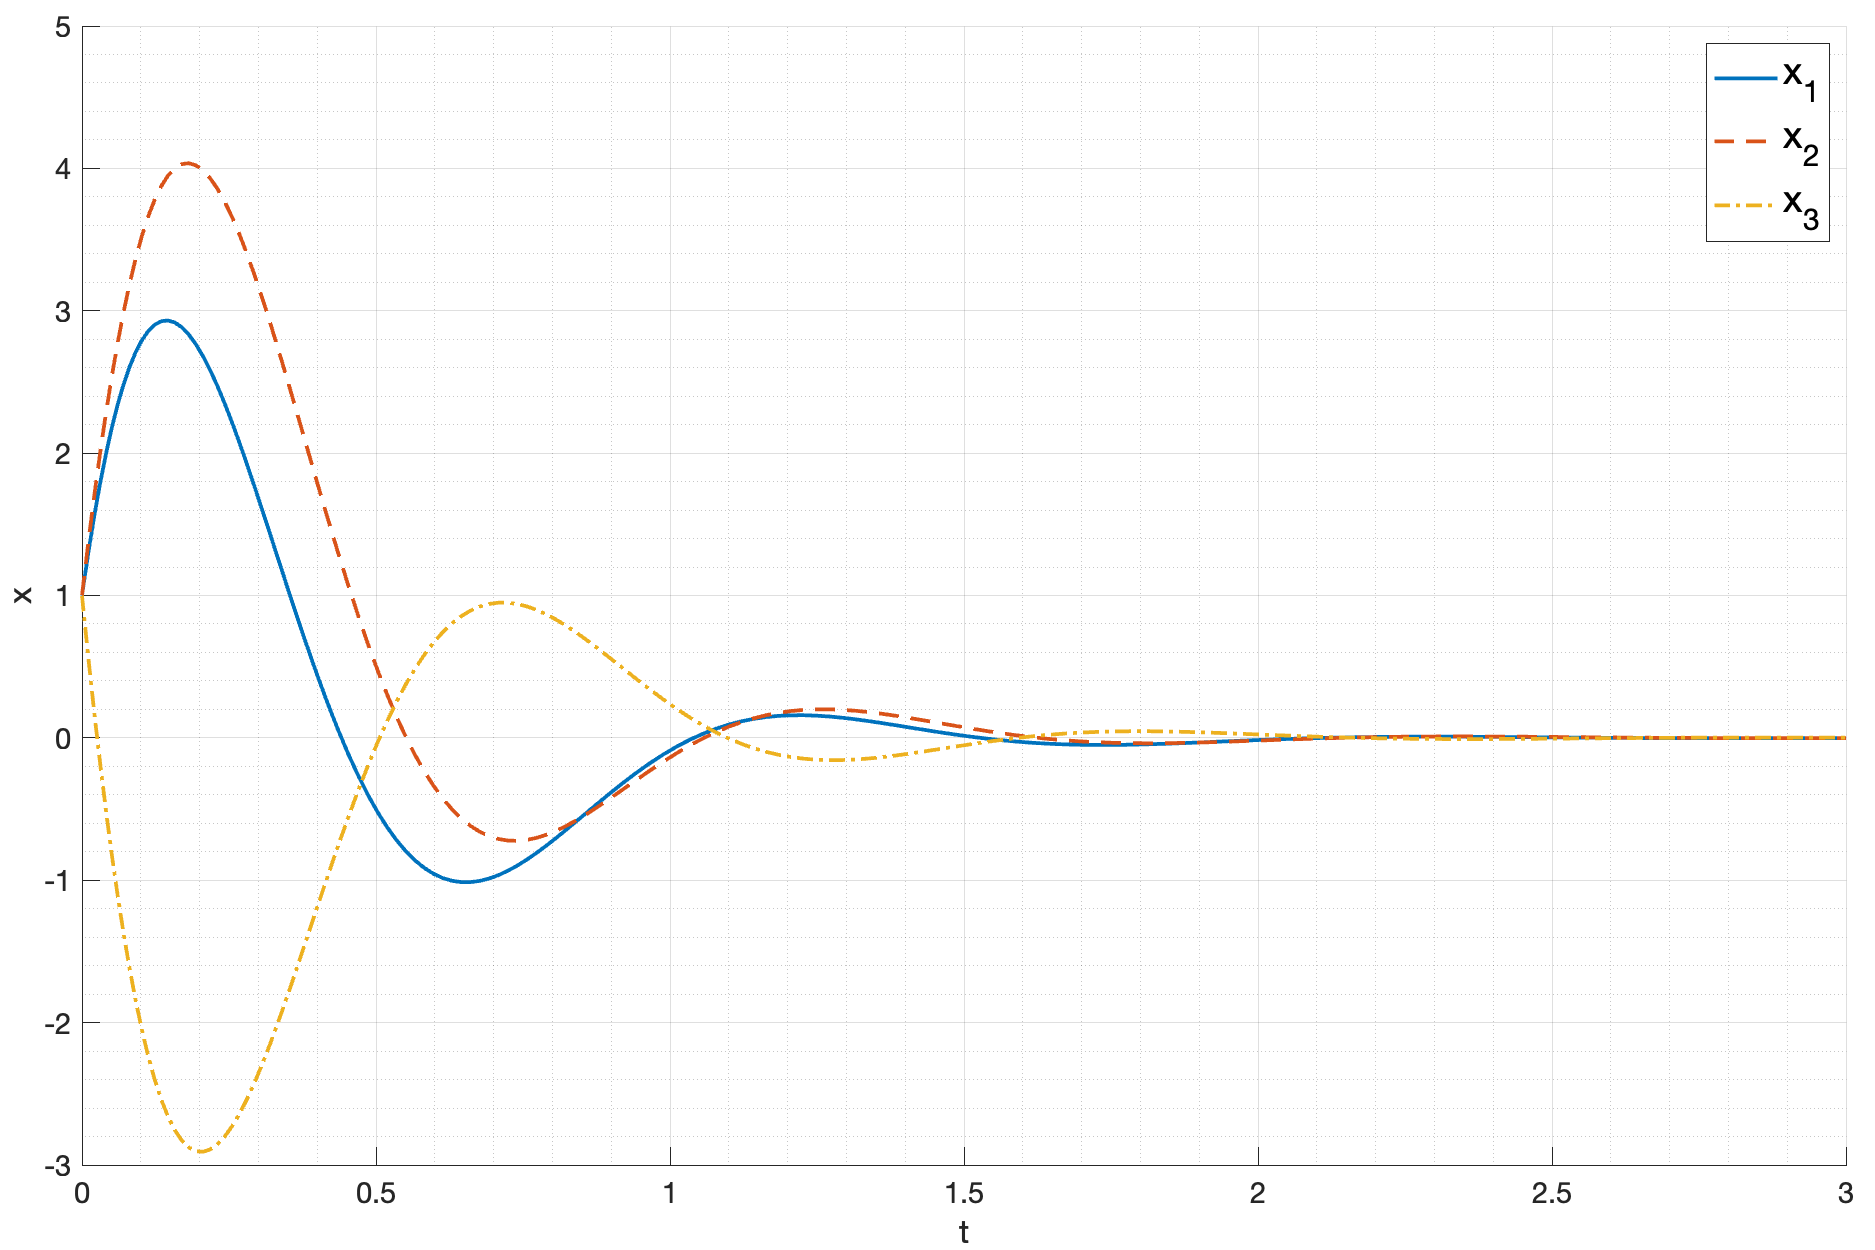
\includegraphics[width=\textwidth]{media/plots/task1_7_x.png}
    \caption{График состояния системы с регулятором $K_5$}
    \label{fig:task1_7_x}
\end{figure}
\begin{figure}[ht!]
    \centering
    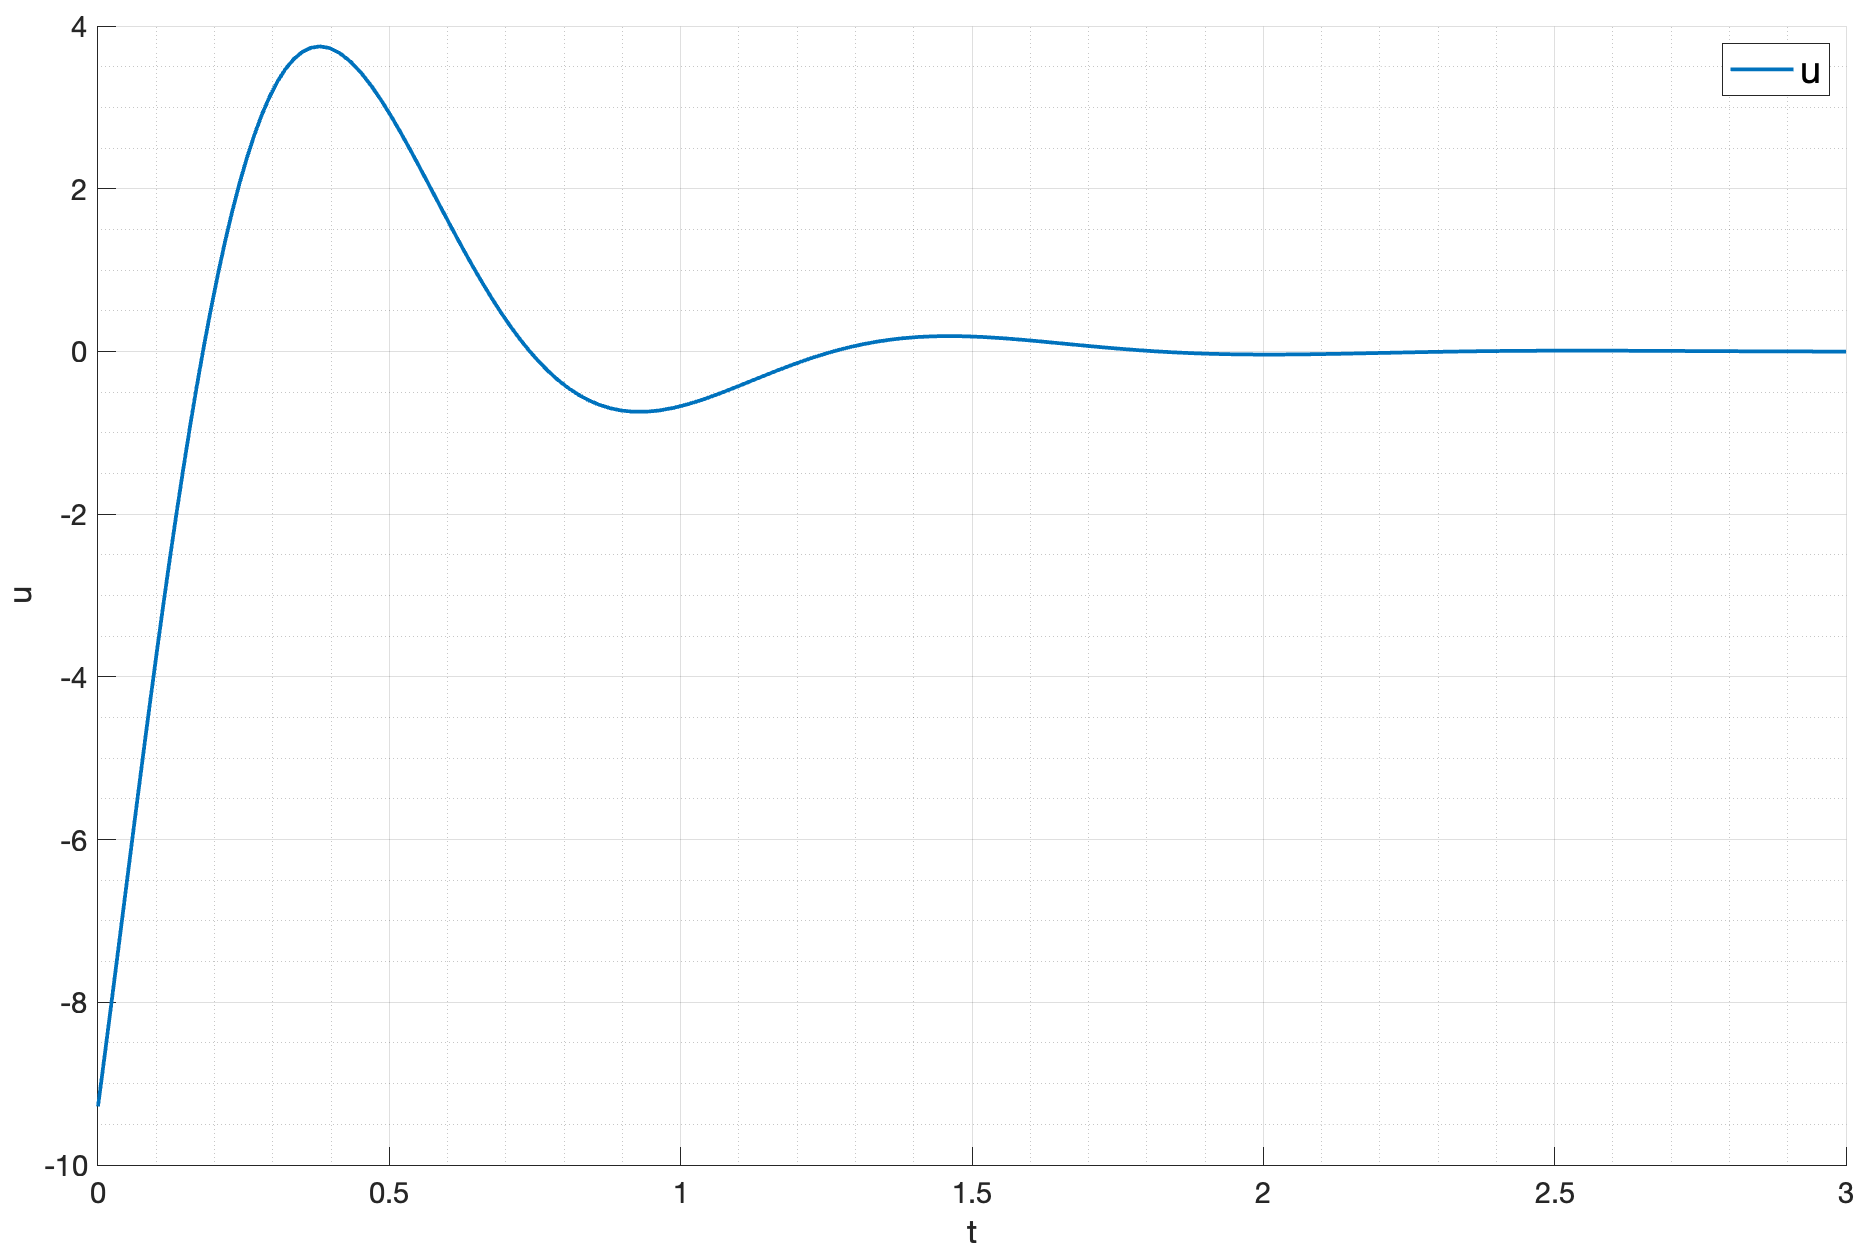
\includegraphics[width=\textwidth]{media/plots/task1_7_u.png}
    \caption{График управления системой с регулятором $K_5$}
    \label{fig:task1_7_u}
\end{figure}
\begin{figure}[ht!]
    \centering
    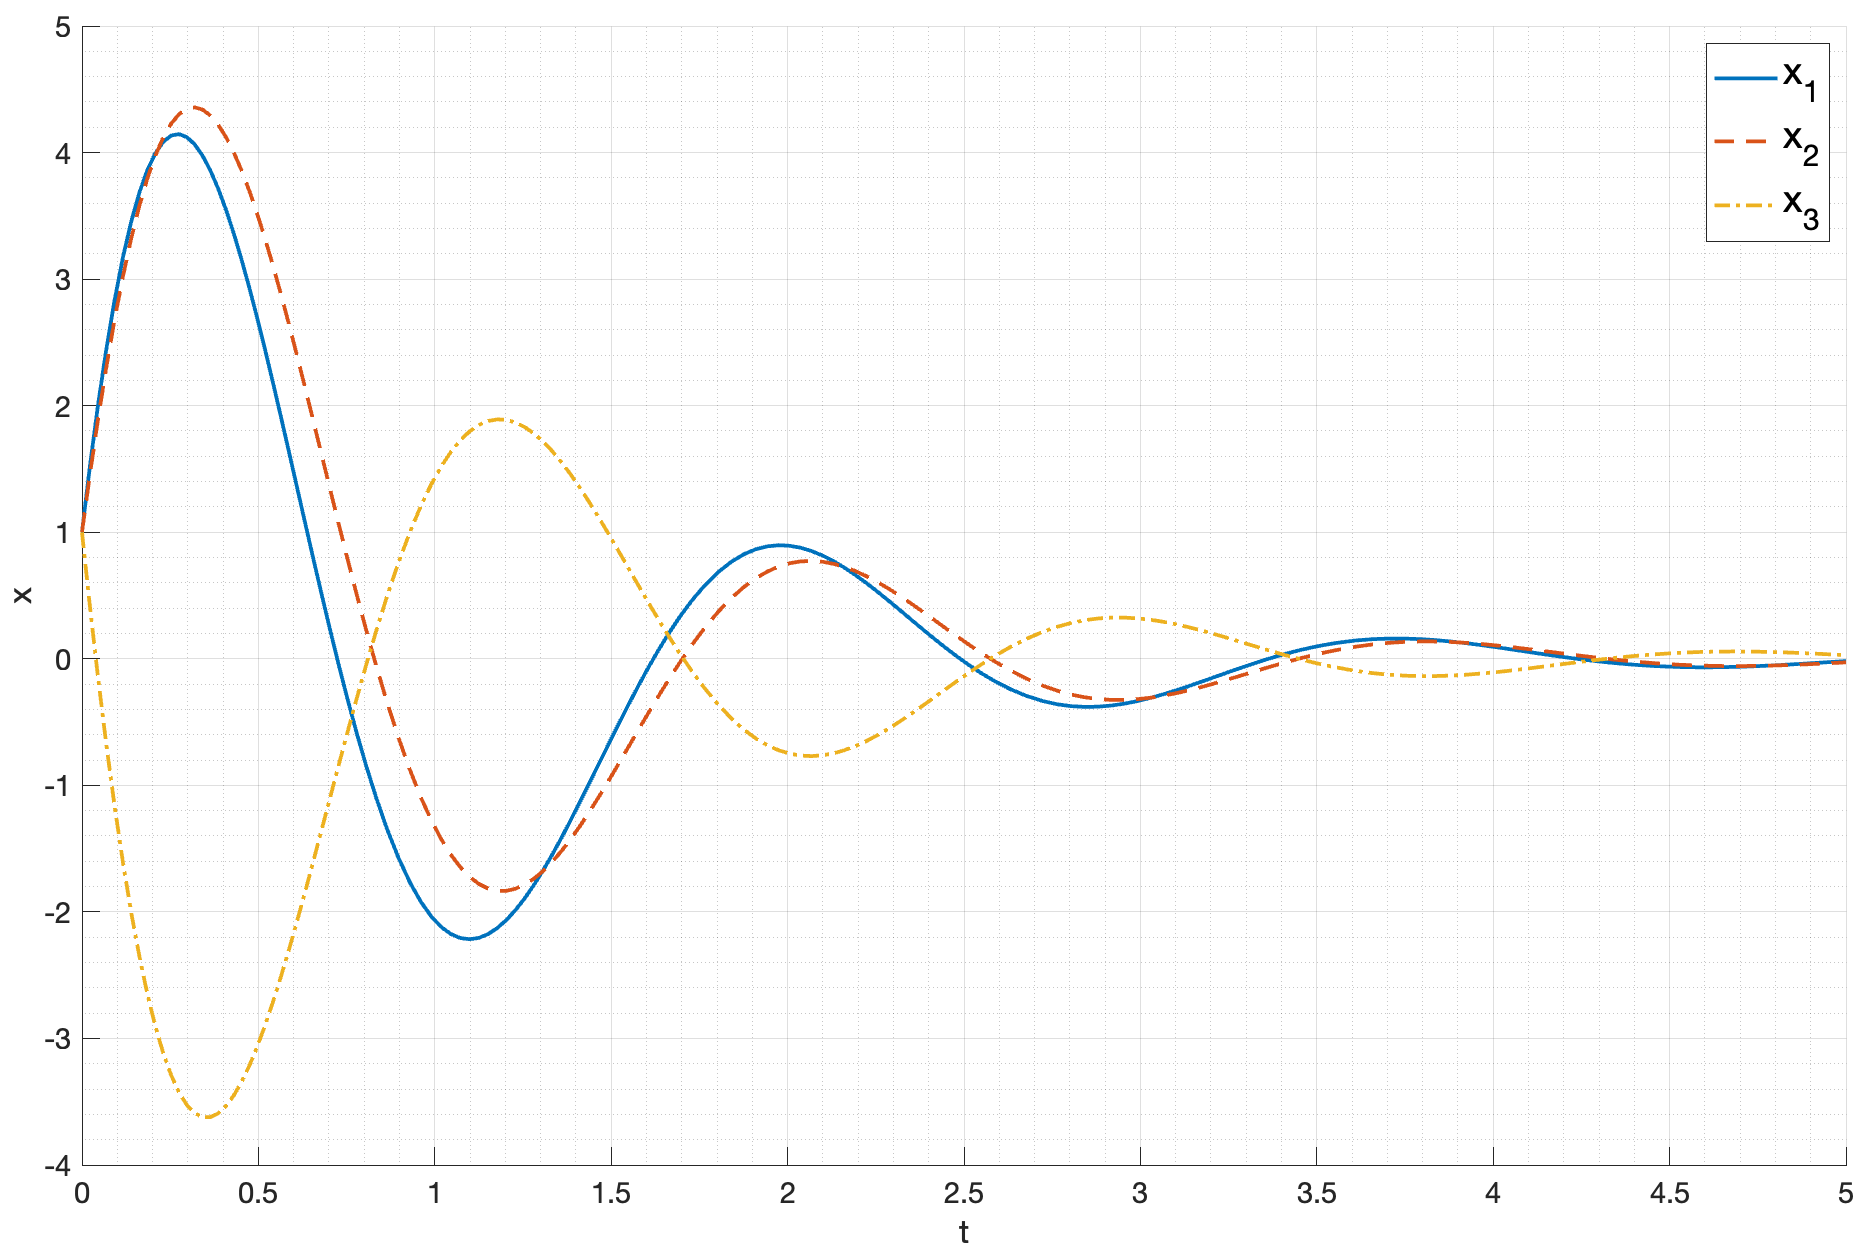
\includegraphics[width=\textwidth]{media/plots/task1_8_x.png}
    \caption{График состояния системы с регулятором $K_6$}
    \label{fig:task1_8_x}
\end{figure}
\begin{figure}[ht!]
    \centering
    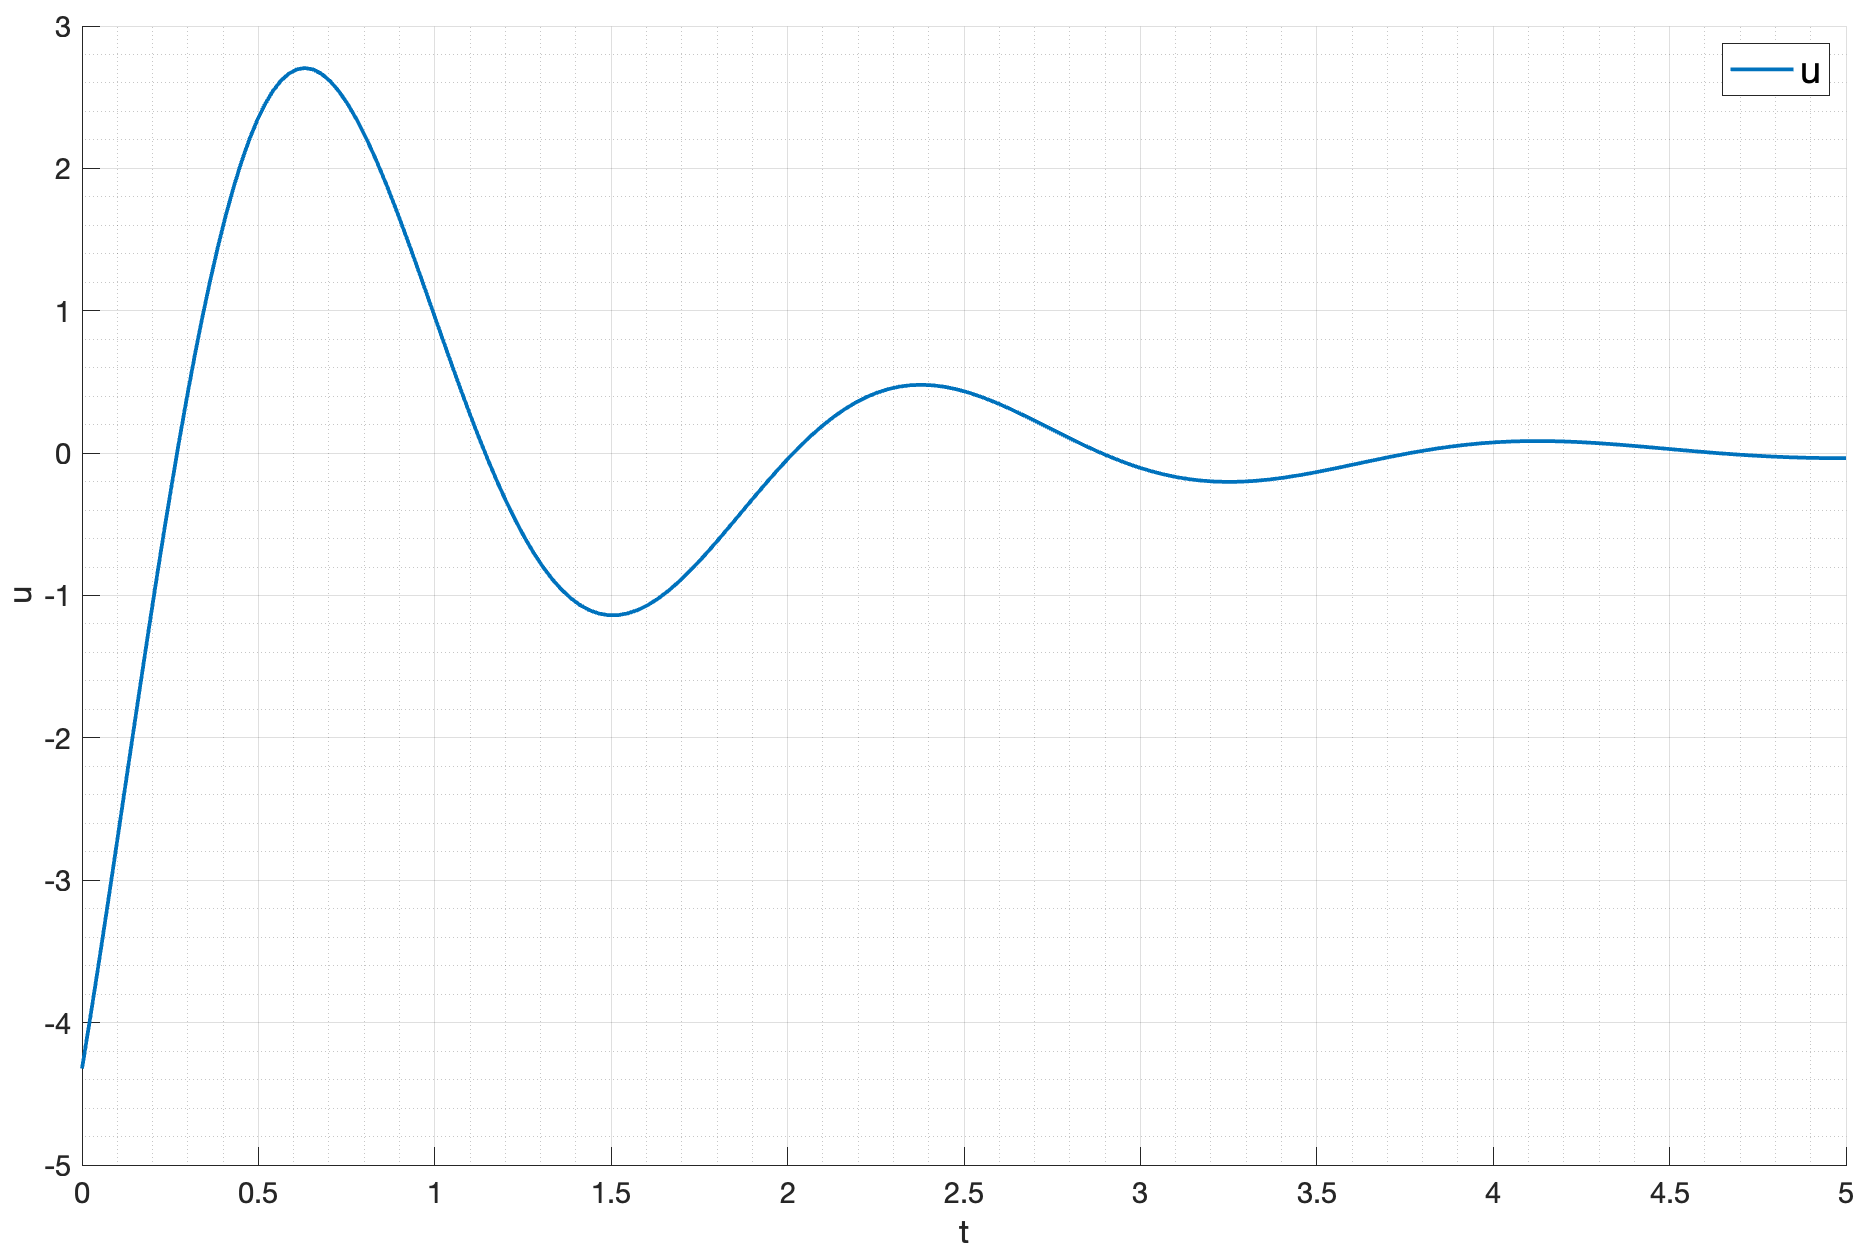
\includegraphics[width=\textwidth]{media/plots/task1_8_u.png}
    \caption{График управления системой с регулятором $K_6$}
    \label{fig:task1_8_u}
\end{figure}

\FloatBarrier
Так же, как и в случае с регуляторами, полученными методом решения матричного неравенства Ляпунова,
можно говорить о том, что чем больше заданная степень устойчивости, тем быстрее система 
сходится к нулю, но при этом управление системы становится больше по модулю. 

При использовании $Q = 0$ в матричном уравнении Риккати, получились регуляторы, 
обеспечивающие заданную степень устойчивости, но не превосходящую ее (кроме неуправляемых собственных чисел).
Таким образом, можно говорить о том, что использование матричного уравнения Риккати
делает управление системы оптимальным. 

\subsection{Выводы}
В ходе рассмотрения регуляторов, обеспечивающих заданную степень устойчивости системы, 
было получено несколько регуляторов, все из которых удовлетворяют заданным условиям.
Но, некоторые из них, без условия минимизации управления, обеспечивают степень устойчивости больше заданной.
Введение условия минимизации управления позволяет добиться оптимального управления системы,
то есть минимального управления, обеспечивающего заданную степень устойчивости системы.
